% Options for packages loaded elsewhere
\PassOptionsToPackage{unicode}{hyperref}
\PassOptionsToPackage{hyphens}{url}
%
\documentclass[
]{article}
\usepackage{amsmath,amssymb}
\usepackage{iftex}
\ifPDFTeX
  \usepackage[T1]{fontenc}
  \usepackage[utf8]{inputenc}
  \usepackage{textcomp} % provide euro and other symbols
\else % if luatex or xetex
  \usepackage{unicode-math} % this also loads fontspec
  \defaultfontfeatures{Scale=MatchLowercase}
  \defaultfontfeatures[\rmfamily]{Ligatures=TeX,Scale=1}
\fi
\usepackage{lmodern}
\ifPDFTeX\else
  % xetex/luatex font selection
\fi
% Use upquote if available, for straight quotes in verbatim environments
\IfFileExists{upquote.sty}{\usepackage{upquote}}{}
\IfFileExists{microtype.sty}{% use microtype if available
  \usepackage[]{microtype}
  \UseMicrotypeSet[protrusion]{basicmath} % disable protrusion for tt fonts
}{}
\makeatletter
\@ifundefined{KOMAClassName}{% if non-KOMA class
  \IfFileExists{parskip.sty}{%
    \usepackage{parskip}
  }{% else
    \setlength{\parindent}{0pt}
    \setlength{\parskip}{6pt plus 2pt minus 1pt}}
}{% if KOMA class
  \KOMAoptions{parskip=half}}
\makeatother
\usepackage{xcolor}
\usepackage[margin=1in]{geometry}
\usepackage{graphicx}
\makeatletter
\def\maxwidth{\ifdim\Gin@nat@width>\linewidth\linewidth\else\Gin@nat@width\fi}
\def\maxheight{\ifdim\Gin@nat@height>\textheight\textheight\else\Gin@nat@height\fi}
\makeatother
% Scale images if necessary, so that they will not overflow the page
% margins by default, and it is still possible to overwrite the defaults
% using explicit options in \includegraphics[width, height, ...]{}
\setkeys{Gin}{width=\maxwidth,height=\maxheight,keepaspectratio}
% Set default figure placement to htbp
\makeatletter
\def\fps@figure{htbp}
\makeatother
\setlength{\emergencystretch}{3em} % prevent overfull lines
\providecommand{\tightlist}{%
  \setlength{\itemsep}{0pt}\setlength{\parskip}{0pt}}
\setcounter{secnumdepth}{-\maxdimen} % remove section numbering
\usepackage{float} \usepackage{booktabs} \usepackage{longtable} \usepackage{array} \usepackage{multirow} \usepackage[table]{xcolor} \usepackage{wrapfig} \floatplacement{figure}{H} \usepackage[normalem]{ulem} \usepackage{float}
\usepackage{booktabs}
\usepackage{longtable}
\usepackage{array}
\usepackage{multirow}
\usepackage{wrapfig}
\usepackage{float}
\usepackage{colortbl}
\usepackage{pdflscape}
\usepackage{tabu}
\usepackage{threeparttable}
\usepackage{threeparttablex}
\usepackage[normalem]{ulem}
\usepackage{makecell}
\usepackage{xcolor}
\usepackage{fontspec}
\usepackage{multicol}
\usepackage{hhline}
\newlength\Oldarrayrulewidth
\newlength\Oldtabcolsep
\usepackage{hyperref}
\usepackage{caption}
\usepackage{anyfontsize}
\ifLuaTeX
  \usepackage{selnolig}  % disable illegal ligatures
\fi
\IfFileExists{bookmark.sty}{\usepackage{bookmark}}{\usepackage{hyperref}}
\IfFileExists{xurl.sty}{\usepackage{xurl}}{} % add URL line breaks if available
\urlstyle{same}
\hypersetup{
  pdftitle={IPMH: Integration of stepped care for perinatal mood and anxiety disorders among women attending MCH clinics},
  hidelinks,
  pdfcreator={LaTeX via pandoc}}

\title{IPMH: Integration of stepped care for perinatal mood and anxiety
disorders among women attending MCH clinics}
\usepackage{etoolbox}
\makeatletter
\providecommand{\subtitle}[1]{% add subtitle to \maketitle
  \apptocmd{\@title}{\par {\large #1 \par}}{}{}
}
\makeatother
\subtitle{Data and Safety Monitoring Board (DSMB): Closed Report}
\author{}
\date{\vspace{-2.5em}28 May 2026}

\begin{document}
\maketitle

\includegraphics[width=1\linewidth]{../../../../OneDrive-UW/IPMH study/Data/IPMH logo}

\newpage

John Kinuthia, MBChD, MMed, MPH, Kenyatta National Hospital

Keshet Ronen, PhD, MPH, University of Washington

Amritha Bhat, MBBS, MD, MPH, University of Washington

Report prepared by: David Owaga \& Yuwei Wang

Date of data freeze: 11 May 2026

\newpage

\tableofcontents

\newpage

\hypertarget{study-summary}{%
\section{1. Study Summary}\label{study-summary}}

\global\setlength{\Oldarrayrulewidth}{\arrayrulewidth}

\global\setlength{\Oldtabcolsep}{\tabcolsep}

\setlength{\tabcolsep}{2pt}

\renewcommand*{\arraystretch}{1.5}



\providecommand{\ascline}[3]{\noalign{\global\arrayrulewidth #1}\arrayrulecolor[HTML]{#2}\cline{#3}}

\begin{longtable}[c]{|p{2.00in}|p{5.00in}}



\ascline{1.5pt}{666666}{1-2}

\multicolumn{1}{>{\raggedright}m{\dimexpr 2in+0\tabcolsep}}{\textcolor[HTML]{000000}{\fontsize{11}{11}\selectfont{\global\setmainfont{Helvetica}{Title}}}} & \multicolumn{1}{!{\color[HTML]{000000}\vrule width 1pt}>{\raggedright}m{\dimexpr 5in+0\tabcolsep}}{\textcolor[HTML]{000000}{\fontsize{11}{11}\selectfont{\global\setmainfont{Helvetica}{IPMH:\ Integration\ of\ stepped\ care\ for\ perinatal\ mood\ and\ anxiety\ disorders\ among\ women\ attending\ MCH\ clinics}}}} \\

\ascline{1.5pt}{666666}{1-2}\endfirsthead 

\ascline{1.5pt}{666666}{1-2}

\multicolumn{1}{>{\raggedright}m{\dimexpr 2in+0\tabcolsep}}{\textcolor[HTML]{000000}{\fontsize{11}{11}\selectfont{\global\setmainfont{Helvetica}{Title}}}} & \multicolumn{1}{!{\color[HTML]{000000}\vrule width 1pt}>{\raggedright}m{\dimexpr 5in+0\tabcolsep}}{\textcolor[HTML]{000000}{\fontsize{11}{11}\selectfont{\global\setmainfont{Helvetica}{IPMH:\ Integration\ of\ stepped\ care\ for\ perinatal\ mood\ and\ anxiety\ disorders\ among\ women\ attending\ MCH\ clinics}}}} \\

\ascline{1.5pt}{666666}{1-2}\endhead



\multicolumn{1}{>{\raggedright}m{\dimexpr 2in+0\tabcolsep}}{\textcolor[HTML]{000000}{\fontsize{11}{11}\selectfont{\global\setmainfont{Helvetica}{Primary\ Objective}}}} & \multicolumn{1}{!{\color[HTML]{000000}\vrule width 1pt}>{\raggedright}m{\dimexpr 5in+0\tabcolsep}}{\textcolor[HTML]{000000}{\fontsize{11}{11}\selectfont{\global\setmainfont{Helvetica}{Integrate\ IPMH,\ a\ stepped\ care\ intervention\ for\ screening\ and\ treatment\ of\ perinatal\ mood\ and\ anxiety\ disorders\ (PMADs),\ and\ its\ implementation\ strategies,\ into\ maternal\ and\ child\ health\ clinics\ and\ pragmatically\ evaluate\ its\ clinical,\ service\ delivery,\ and\ implementation\ outcomes}}}} \\





\multicolumn{1}{>{\raggedright}m{\dimexpr 2in+0\tabcolsep}}{\textcolor[HTML]{000000}{\fontsize{11}{11}\selectfont{\global\setmainfont{Helvetica}{Study\ Design}}}} & \multicolumn{1}{!{\color[HTML]{000000}\vrule width 1pt}>{\raggedright}m{\dimexpr 5in+0\tabcolsep}}{\textcolor[HTML]{000000}{\fontsize{11}{11}\selectfont{\global\setmainfont{Helvetica}{A\ 2-arm,\ non-blinded\ cluster\ randomized\ controlled\ trial\ (RCT)\ comparing\ the\ effect\ of\ IPMH\ and\ associated\ implementation\ strategies\ on\ depression,\ anxiety,\ quality\ of\ life,\ and\ adverse\ perinatal\ outcomes\ vs.\ control\ (standard\ of\ care)\ among\ Kenyan\ women}}}} \\





\multicolumn{1}{>{\raggedright}m{\dimexpr 2in+0\tabcolsep}}{\textcolor[HTML]{000000}{\fontsize{11}{11}\selectfont{\global\setmainfont{Helvetica}{Study\ Population}}}} & \multicolumn{1}{!{\color[HTML]{000000}\vrule width 1pt}>{\raggedright}m{\dimexpr 5in+0\tabcolsep}}{\textcolor[HTML]{000000}{\fontsize{11}{11}\selectfont{\global\setmainfont{Helvetica}{Pregnant\ Kenyan\ women}}}} \\





\multicolumn{1}{>{\raggedright}m{\dimexpr 2in+0\tabcolsep}}{\textcolor[HTML]{000000}{\fontsize{11}{11}\selectfont{\global\setmainfont{Helvetica}{Inclusion\ Criteria}}}} & \multicolumn{1}{!{\color[HTML]{000000}\vrule width 1pt}>{\raggedright}m{\dimexpr 5in+0\tabcolsep}}{\textcolor[HTML]{000000}{\fontsize{11}{11}\selectfont{\global\setmainfont{Helvetica}{-Receiving\ antenatal\ care\ at\ study\ facility}}}\textcolor[HTML]{000000}{\fontsize{11}{11}\selectfont{\global\setmainfont{Helvetica}{\linebreak }}}\textcolor[HTML]{000000}{\fontsize{11}{11}\selectfont{\global\setmainfont{Helvetica}{->=20\ weeks\ gestation}}}\textcolor[HTML]{000000}{\fontsize{11}{11}\selectfont{\global\setmainfont{Helvetica}{\linebreak }}}\textcolor[HTML]{000000}{\fontsize{11}{11}\selectfont{\global\setmainfont{Helvetica}{-Age>=14}}}\textcolor[HTML]{000000}{\fontsize{11}{11}\selectfont{\global\setmainfont{Helvetica}{\linebreak }}}\textcolor[HTML]{000000}{\fontsize{11}{11}\selectfont{\global\setmainfont{Helvetica}{-screen\ positive\ for\ PMAD\ symptoms\ (PHQ-2>=3\ and/or\ GAD-2>=3)}}}} \\





\multicolumn{1}{>{\raggedright}m{\dimexpr 2in+0\tabcolsep}}{\textcolor[HTML]{000000}{\fontsize{11}{11}\selectfont{\global\setmainfont{Helvetica}{Target\ Sample\ Size}}}} & \multicolumn{1}{!{\color[HTML]{000000}\vrule width 1pt}>{\raggedright}m{\dimexpr 5in+0\tabcolsep}}{\textcolor[HTML]{000000}{\fontsize{11}{11}\selectfont{\global\setmainfont{Helvetica}{2970,\ including\ 405\ women\ living\ with\ HIV\ (WLWH)}}}} \\





\multicolumn{1}{>{\raggedright}m{\dimexpr 2in+0\tabcolsep}}{\textcolor[HTML]{000000}{\fontsize{11}{11}\selectfont{\global\setmainfont{Helvetica}{Actual\ Enrollment}}}} & \multicolumn{1}{!{\color[HTML]{000000}\vrule width 1pt}>{\raggedright}m{\dimexpr 5in+0\tabcolsep}}{\textcolor[HTML]{000000}{\fontsize{11}{11}\selectfont{\global\setmainfont{Helvetica}{2383}}}} \\





\multicolumn{1}{>{\raggedright}m{\dimexpr 2in+0\tabcolsep}}{\textcolor[HTML]{000000}{\fontsize{11}{11}\selectfont{\global\setmainfont{Helvetica}{Participants\ Completed\ Follow-up}}}} & \multicolumn{1}{!{\color[HTML]{000000}\vrule width 1pt}>{\raggedright}m{\dimexpr 5in+0\tabcolsep}}{\textcolor[HTML]{000000}{\fontsize{11}{11}\selectfont{\global\setmainfont{Helvetica}{960}}}} \\





\multicolumn{1}{>{\raggedright}m{\dimexpr 2in+0\tabcolsep}}{\textcolor[HTML]{000000}{\fontsize{11}{11}\selectfont{\global\setmainfont{Helvetica}{Duration}}}} & \multicolumn{1}{!{\color[HTML]{000000}\vrule width 1pt}>{\raggedright}m{\dimexpr 5in+0\tabcolsep}}{\textcolor[HTML]{000000}{\fontsize{11}{11}\selectfont{\global\setmainfont{Helvetica}{Follow-up\ through\ 6\ months\ postpartum}}}} \\





\multicolumn{1}{>{\raggedright}m{\dimexpr 2in+0\tabcolsep}}{\textcolor[HTML]{000000}{\fontsize{11}{11}\selectfont{\global\setmainfont{Helvetica}{Date\ Study\ Open}}}} & \multicolumn{1}{!{\color[HTML]{000000}\vrule width 1pt}>{\raggedright}m{\dimexpr 5in+0\tabcolsep}}{\textcolor[HTML]{000000}{\fontsize{11}{11}\selectfont{\global\setmainfont{Helvetica}{September\ 19,\ 2023}}}} \\





\multicolumn{1}{>{\raggedright}m{\dimexpr 2in+0\tabcolsep}}{\textcolor[HTML]{000000}{\fontsize{11}{11}\selectfont{\global\setmainfont{Helvetica}{Date\ of\ First\ Complete\ Enrollment}}}} & \multicolumn{1}{!{\color[HTML]{000000}\vrule width 1pt}>{\raggedright}m{\dimexpr 5in+0\tabcolsep}}{\textcolor[HTML]{000000}{\fontsize{11}{11}\selectfont{\global\setmainfont{Helvetica}{February\ 17,\ 2025}}}} \\





\multicolumn{1}{>{\raggedright}m{\dimexpr 2in+0\tabcolsep}}{\textcolor[HTML]{000000}{\fontsize{11}{11}\selectfont{\global\setmainfont{Helvetica}{Estimated\ End\ of\ Study}}}} & \multicolumn{1}{!{\color[HTML]{000000}\vrule width 1pt}>{\raggedright}m{\dimexpr 5in+0\tabcolsep}}{\textcolor[HTML]{000000}{\fontsize{11}{11}\selectfont{\global\setmainfont{Helvetica}{July\ 31,\ 2028}}}} \\





\multicolumn{1}{>{\raggedright}m{\dimexpr 2in+0\tabcolsep}}{\textcolor[HTML]{000000}{\fontsize{11}{11}\selectfont{\global\setmainfont{Helvetica}{Endpoints}}}} & \multicolumn{1}{!{\color[HTML]{000000}\vrule width 1pt}>{\raggedright}m{\dimexpr 5in+0\tabcolsep}}{\textcolor[HTML]{000000}{\fontsize{11}{11}\selectfont{\global\setmainfont{Helvetica}{Primary:\ Depression\ (Patient\ Health\ Questionnaire-9\ [PHQ-9]\ score)\ and\ anxiety\ (Generalized\ Anxiety\ Disorder-7\ [GAD-7]\ score)}}}} \\





\multicolumn{1}{>{\raggedright}m{\dimexpr 2in+0\tabcolsep}}{\textcolor[HTML]{000000}{\fontsize{11}{11}\selectfont{\global\setmainfont{Helvetica}{}}}} & \multicolumn{1}{!{\color[HTML]{000000}\vrule width 1pt}>{\raggedright}m{\dimexpr 5in+0\tabcolsep}}{\textcolor[HTML]{000000}{\fontsize{11}{11}\selectfont{\global\setmainfont{Helvetica}{Secondary:}}}\textcolor[HTML]{000000}{\fontsize{11}{11}\selectfont{\global\setmainfont{Helvetica}{\linebreak }}}\textcolor[HTML]{000000}{\fontsize{11}{11}\selectfont{\global\setmainfont{Helvetica}{-Problem\ Management\ Plus\ (PM+)\ Skill\ Acquisition\ (Reducing\ Tension\ Checklist\ score)}}}\textcolor[HTML]{000000}{\fontsize{11}{11}\selectfont{\global\setmainfont{Helvetica}{\linebreak }}}\textcolor[HTML]{000000}{\fontsize{11}{11}\selectfont{\global\setmainfont{Helvetica}{-Quality\ of\ Life\ (World\ Health\ Organization\ Quality\ of\ Life\ [WHOQOL-BREF]\ score)}}}\textcolor[HTML]{000000}{\fontsize{11}{11}\selectfont{\global\setmainfont{Helvetica}{\linebreak }}}\textcolor[HTML]{000000}{\fontsize{11}{11}\selectfont{\global\setmainfont{Helvetica}{-Any\ adverse\ pregnancy\ outcome}}}} \\

\ascline{1.5pt}{666666}{1-2}



\end{longtable}



\arrayrulecolor[HTML]{000000}

\global\setlength{\arrayrulewidth}{\Oldarrayrulewidth}

\global\setlength{\tabcolsep}{\Oldtabcolsep}

\renewcommand*{\arraystretch}{1}

\newpage

\hypertarget{study-enrollment}{%
\section{2. Study Enrollment}\label{study-enrollment}}

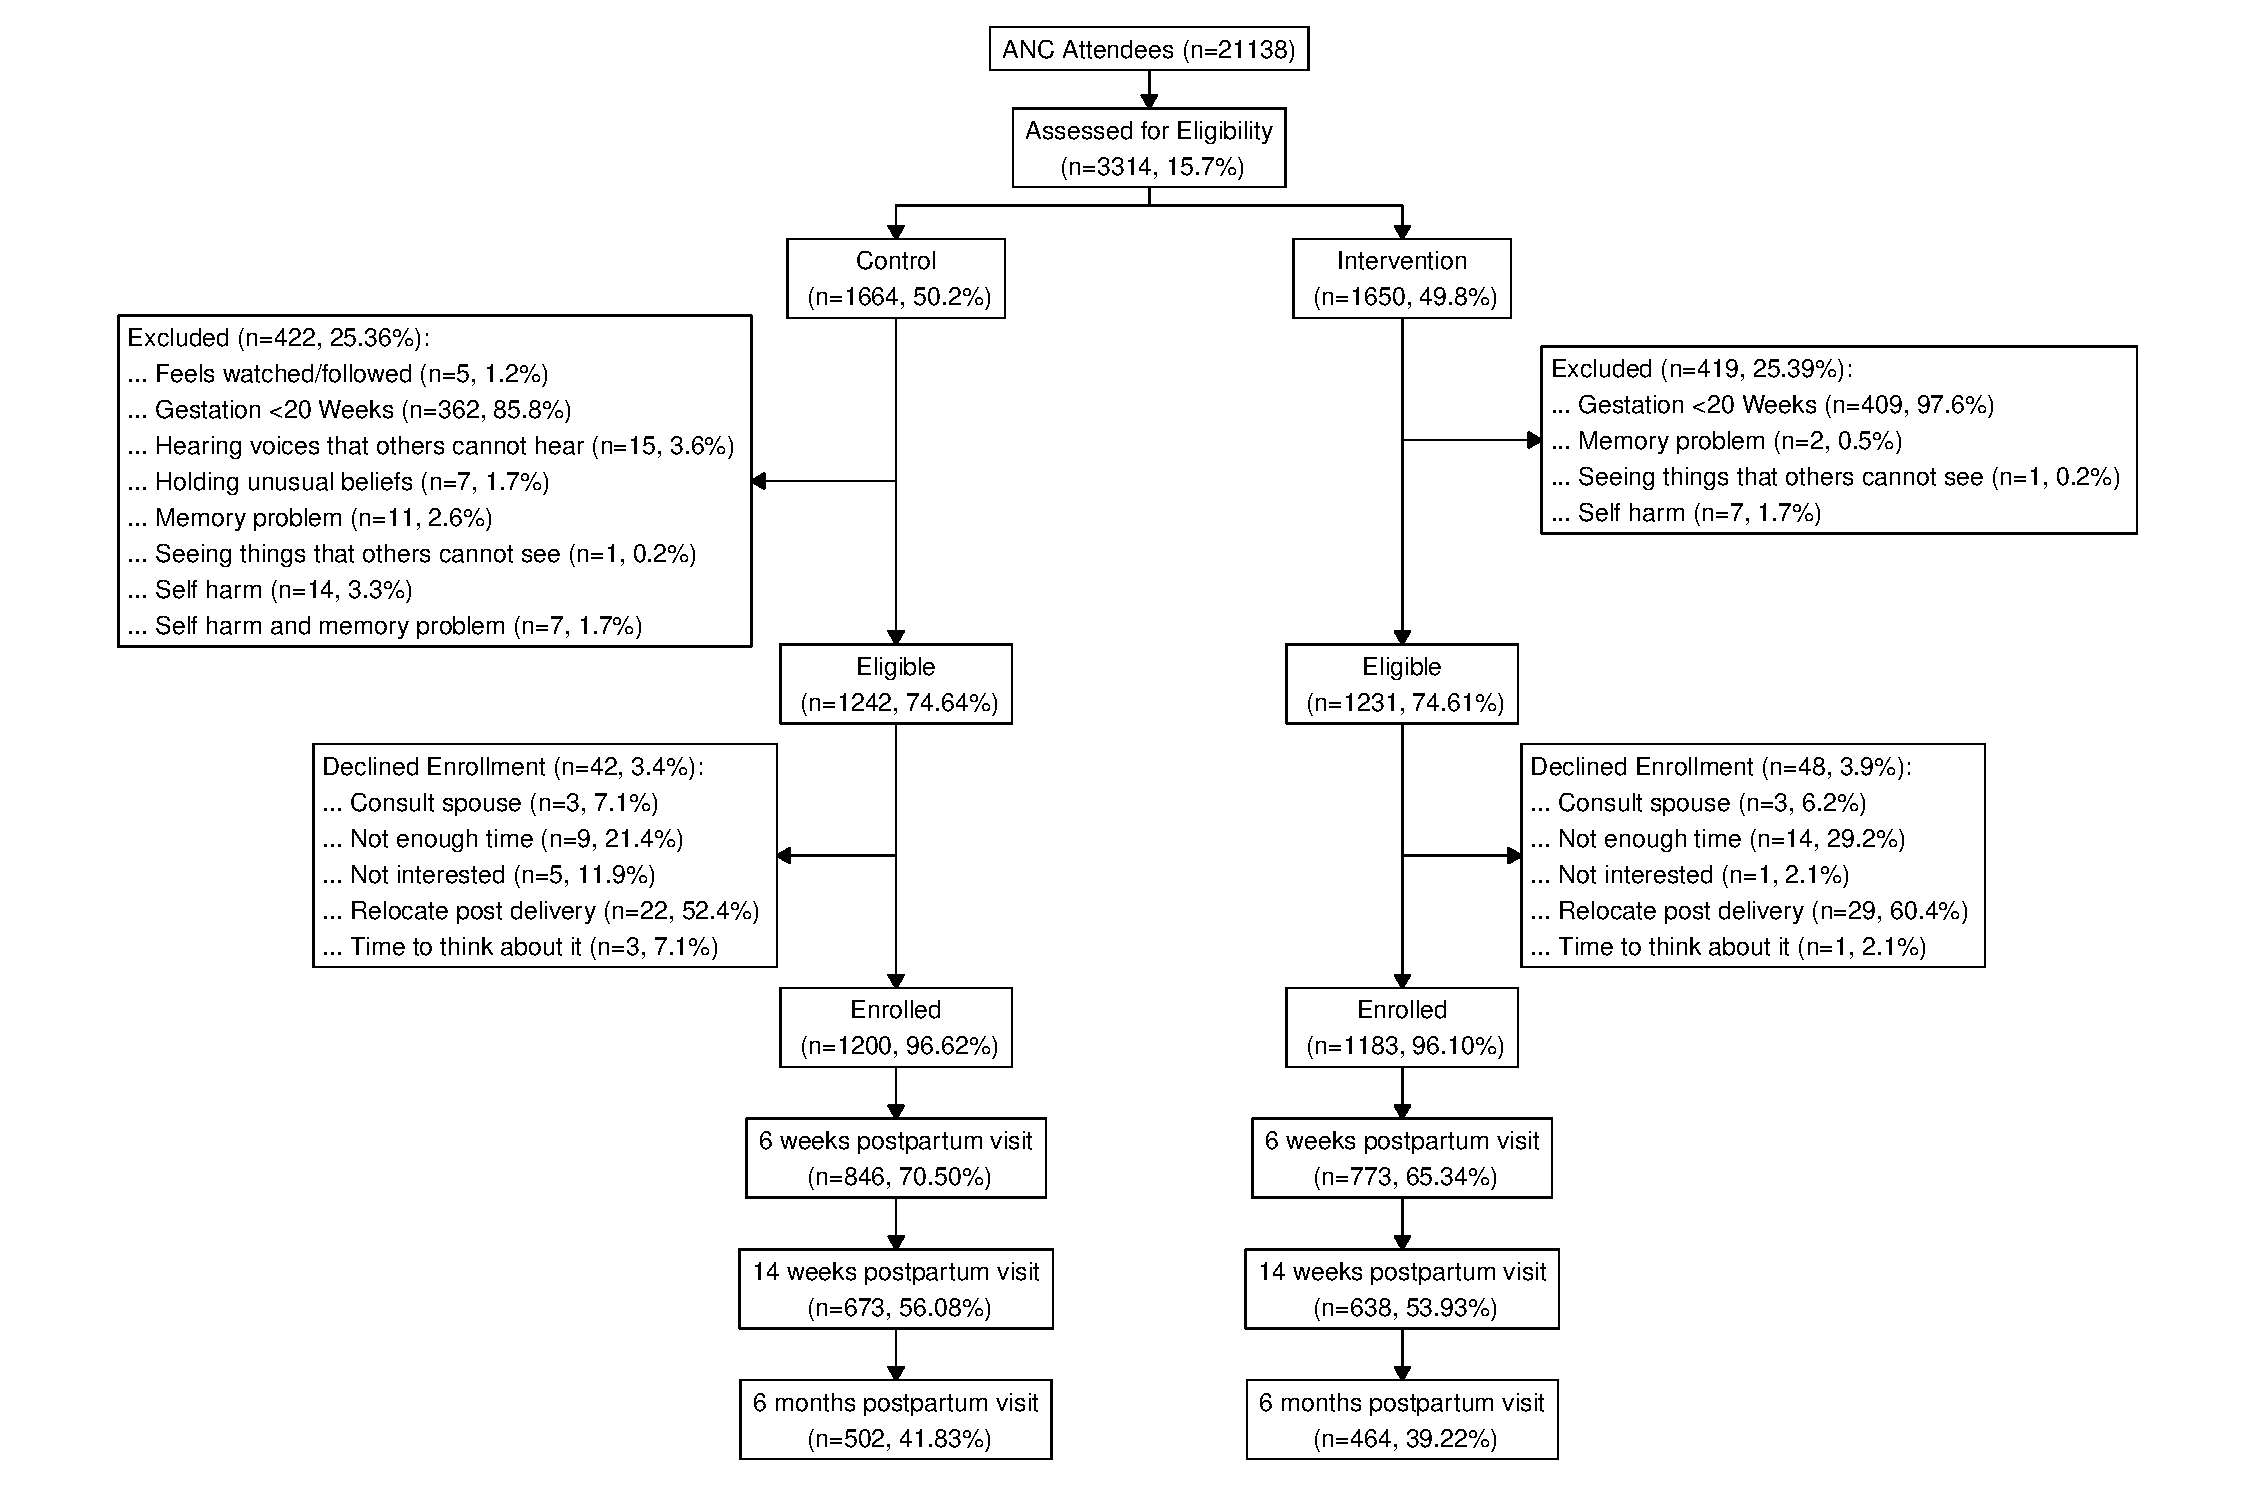
\includegraphics{dsmb_closedreport_jun2026_files/figure-latex/consort diagram-1.pdf}

\newpage

\hypertarget{enrollment-progress---overall}{%
\subsection{2.1 Enrollment Progress -
Overall}\label{enrollment-progress---overall}}

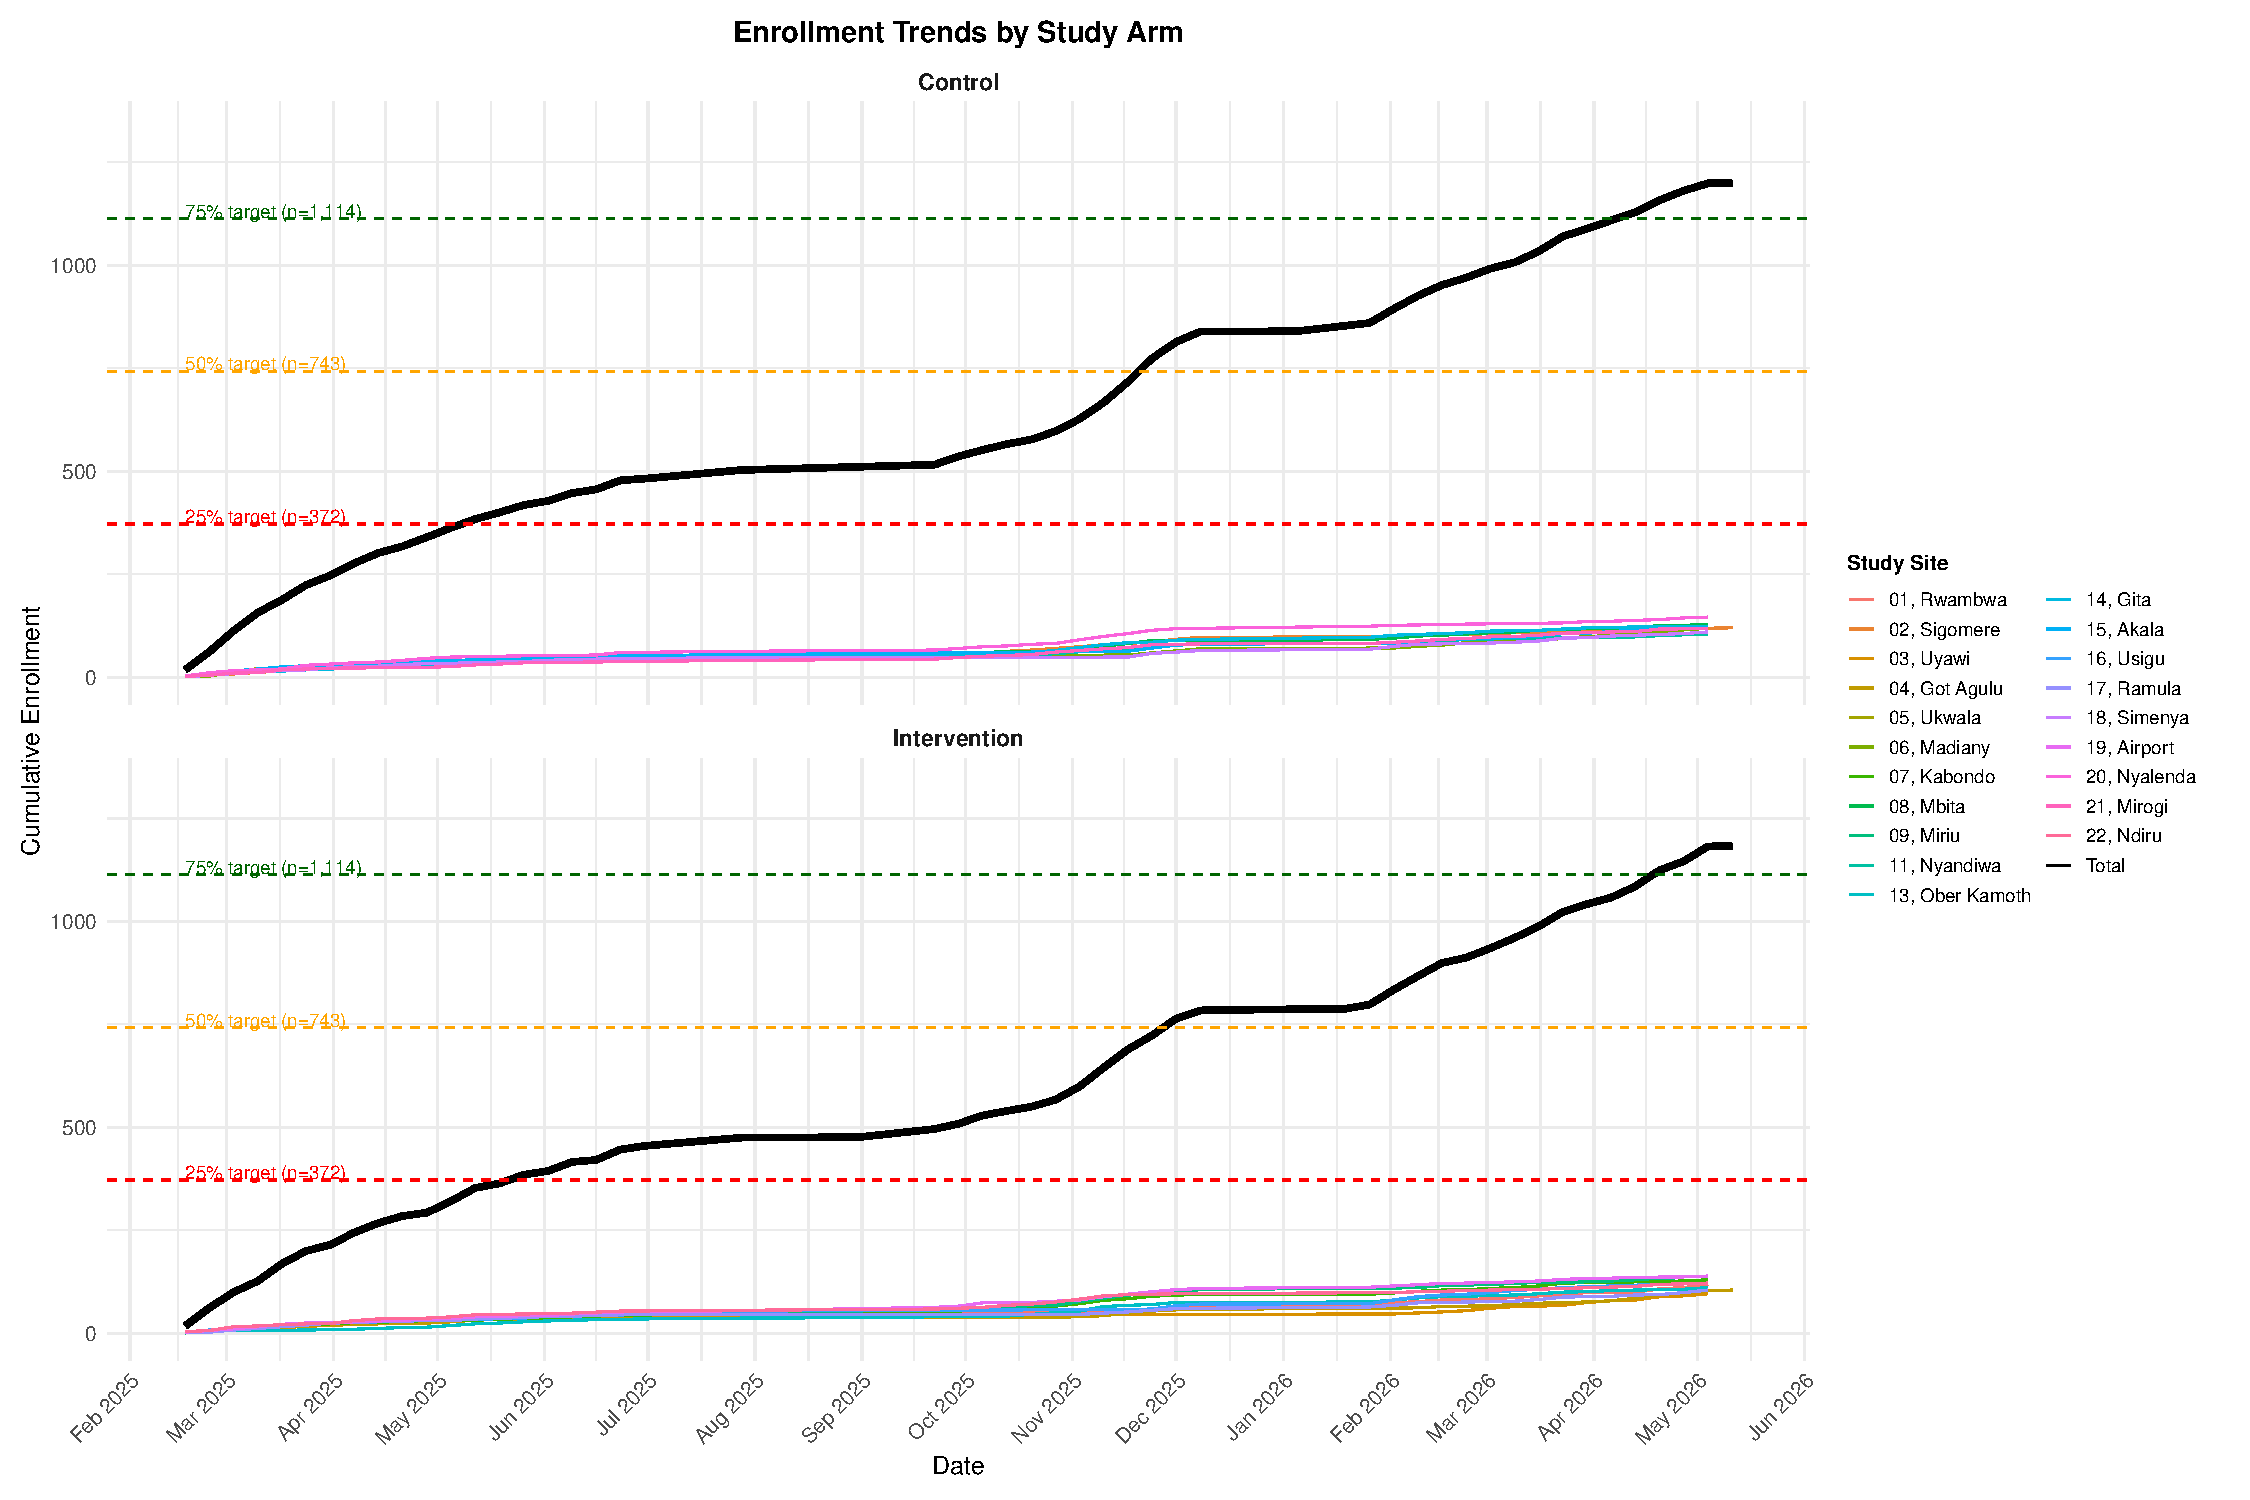
\includegraphics{dsmb_closedreport_jun2026_files/figure-latex/enrollment_progress plot-1.pdf}

\newpage

\hypertarget{enrollment-progress---per-facility}{%
\subsection{2.2 Enrollment Progress - Per
Facility}\label{enrollment-progress---per-facility}}

All 20 facilities have surpassed the 50\% enrollment milestone, each
enrolling at least 74 perinatal women. Progress has continued steadily,
with 20 facilities surpassing the 75\% milestone (\textgreater=111
enrollments), demonstrating strong momentum toward full recruitment.

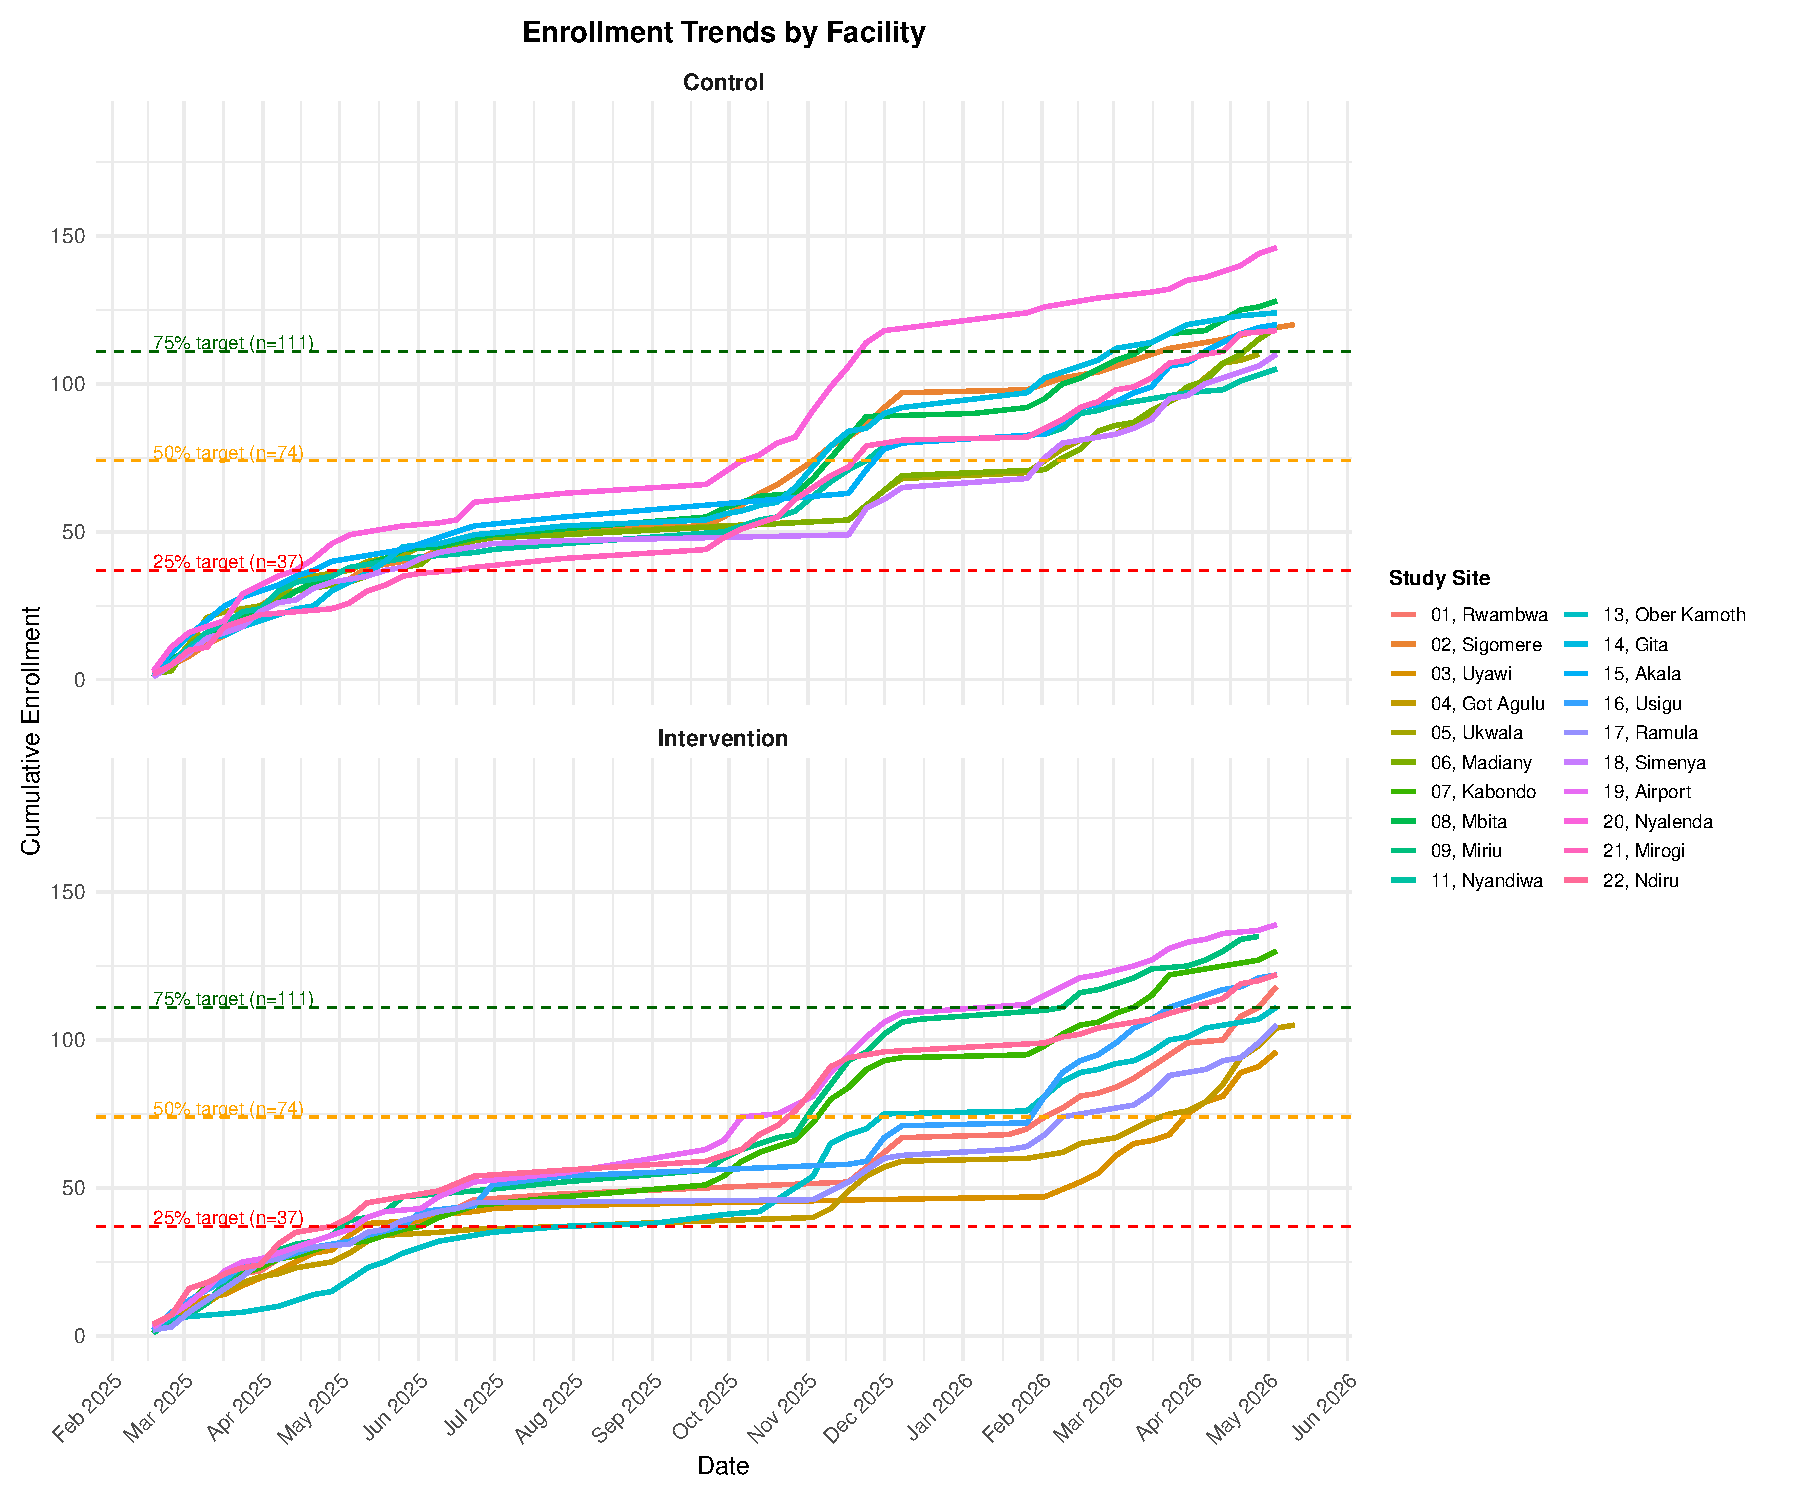
\includegraphics{dsmb_closedreport_jun2026_files/figure-latex/enrollment_sub_facility-1.pdf}

\newpage

\hypertarget{women-living-with-hiv-cohort}{%
\section{3. Women Living with HIV
Cohort}\label{women-living-with-hiv-cohort}}

Overall 2383 participants have been enrolled into the study, of which
361 women are living with HIV (WLHIV), accounting to 15.1\% of total
enrollments. Of these, 215 (59.6\%) have completed their 6 weeks, 170
(47.1\%) have completed 14 weeks, and 118 (32.7\%) have completed their
6 months postpartum follow-up visits. Percentages do not reflect study
retention as not all enrolled participants have reached follow-up
visits.

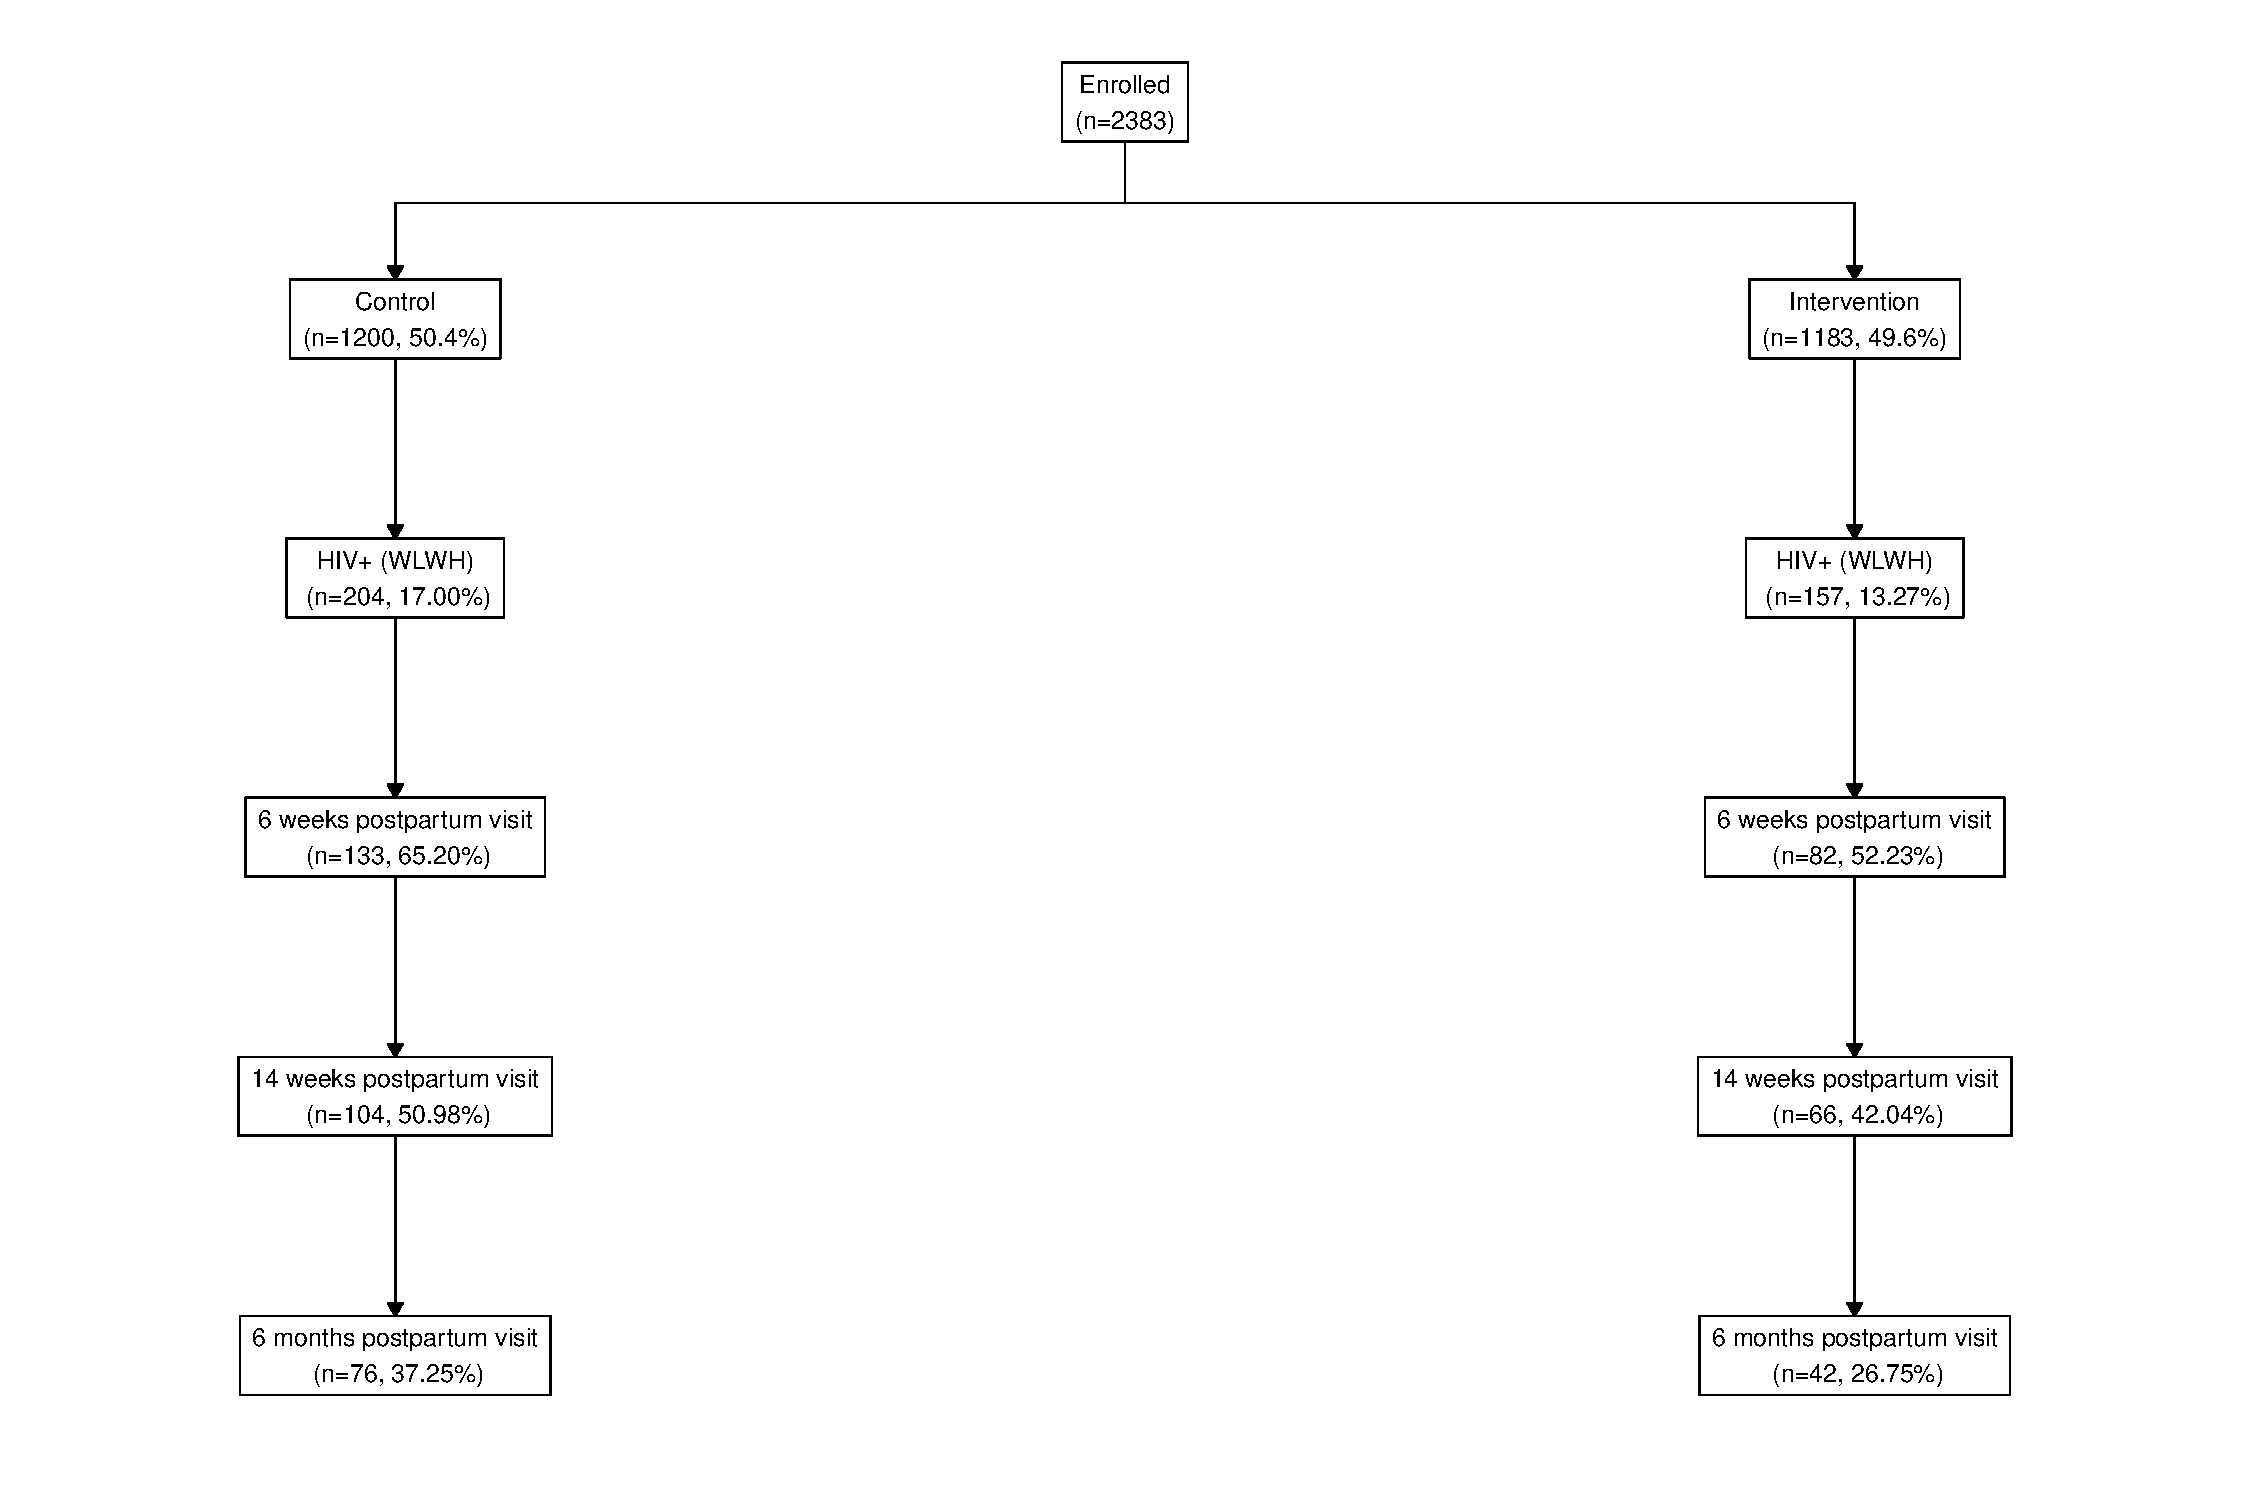
\includegraphics{dsmb_closedreport_jun2026_files/figure-latex/consort_WLWHIV-1.pdf}

\newpage

\hypertarget{ineligibility}{%
\section{4. Ineligibility}\label{ineligibility}}

Women were ineligible if their gestational age at eligibility assessment
was \textless20 weeks, if they endorsed thoughts/actions of self-harm,
and if they endorsed symptoms of potential psychosis (e.g., hearing
voices that others cannot hear, holding unusual beliefs, or feeling
watched/followed), or if they endorsed experiencing memory problems.

\setcounter{table}{0}

\begin{table}[H]
\centering
\caption{\label{tab:ineligibility}Summary of Study Ineligibility by Arm}
\centering
\resizebox{\ifdim\width>\linewidth\linewidth\else\width\fi}{!}{
\fontsize{10}{12}\selectfont
\begin{tabular}[t]{lccc}
\toprule
\textbf{Characteristic} & \makecell[c]{\textbf{Control}\ \ \\N = 422} & \makecell[c]{\textbf{Intervention}\ \ \\N = 419} & \makecell[c]{\textbf{Overall}\ \ \\N = 841}\\
\midrule
\cellcolor{gray!10}{\textbf{Reasons for Ineligibility}} & \cellcolor{gray!10}{} & \cellcolor{gray!10}{} & \cellcolor{gray!10}{}\\
\hspace{1em}Gestation <20 Weeks & 362 (86\%) & 409 (98\%) & 771 (92\%)\\
\cellcolor{gray!10}{\hspace{1em}Self harm} & \cellcolor{gray!10}{14 (3.3\%)} & \cellcolor{gray!10}{7 (1.7\%)} & \cellcolor{gray!10}{21 (2.5\%)}\\
\hspace{1em}Hearing voices that others cannot hear & 15 (3.6\%) & 0 (0\%) & 15 (1.8\%)\\
\cellcolor{gray!10}{\hspace{1em}Memory problem} & \cellcolor{gray!10}{11 (2.6\%)} & \cellcolor{gray!10}{2 (0.5\%)} & \cellcolor{gray!10}{13 (1.5\%)}\\
\addlinespace
\hspace{1em}Holding unusual beliefs & 7 (1.7\%) & 0 (0\%) & 7 (0.8\%)\\
\cellcolor{gray!10}{\hspace{1em}Self harm and memory problem} & \cellcolor{gray!10}{7 (1.7\%)} & \cellcolor{gray!10}{0 (0\%)} & \cellcolor{gray!10}{7 (0.8\%)}\\
\hspace{1em}Feels watched/followed & 5 (1.2\%) & 0 (0\%) & 5 (0.6\%)\\
\cellcolor{gray!10}{\hspace{1em}Seeing things that others cannot see} & \cellcolor{gray!10}{1 (0.2\%)} & \cellcolor{gray!10}{1 (0.2\%)} & \cellcolor{gray!10}{2 (0.2\%)}\\
\bottomrule
\multicolumn{4}{l}{\rule{0pt}{1em}\textsuperscript{1} n (\%)}\\
\end{tabular}}
\end{table}

\newpage

\hypertarget{baseline-demographics}{%
\section{5. Baseline Demographics}\label{baseline-demographics}}

\hypertarget{participant-baseline-demographics}{%
\subsection{5.1 Participant Baseline
Demographics}\label{participant-baseline-demographics}}

Demographic characteristics were balanced across study arms, supporting
baseline comparability.

\begin{table}[H]
\centering
\caption{\label{tab:demographics prep}Basic Demographic Summary}
\centering
\resizebox{\ifdim\width>\linewidth\linewidth\else\width\fi}{!}{
\fontsize{8}{10}\selectfont
\begin{tabular}[t]{>{\raggedright\arraybackslash}p{5cm}>{\centering\arraybackslash}p{2.5cm}>{\centering\arraybackslash}p{2.5cm}>{\centering\arraybackslash}p{2.5cm}c}
\toprule
\begingroup\fontsize{9}{11}\selectfont \textbf{\textbf{Characteristic}}\endgroup & \begingroup\fontsize{9}{11}\selectfont \textbf{\textbf{N}}\endgroup & \begingroup\fontsize{9}{11}\selectfont \textbf{\textbf{Control}\ \ \newline N = 1,201}\endgroup & \begingroup\fontsize{9}{11}\selectfont \textbf{\textbf{Intervention}\ \ \newline N = 1,182}\endgroup & \begingroup\fontsize{9}{11}\selectfont \textbf{\makecell[c]{\textbf{Overall}\ \ \\N = 2,383}}\endgroup\\
\midrule
\cellcolor{gray!10}{\textbf{Age (Years)}} & \cellcolor{gray!10}{2,383} & \cellcolor{gray!10}{26.0 [IQR: 21.0, 31.0]} & \cellcolor{gray!10}{25.0 [IQR: 21.0, 30.0]} & \cellcolor{gray!10}{26.0 [IQR: 21.0, 31.0]}\\
\textbf{Do you currently have a partner (Yes)} & 2,383 & 1,037 (86.3\%) & 983 (83.2\%) & 2,020 (84.8\%)\\
\cellcolor{gray!10}{\textbf{Currently Married (Yes)}} & \cellcolor{gray!10}{2,375} & \cellcolor{gray!10}{938 (78.6\%)} & \cellcolor{gray!10}{882 (74.7\%)} & \cellcolor{gray!10}{1,820 (76.6\%)}\\
\textbf{Marriage (Monogamous)} & 1,820 & 831 (88.6\%) & 770 (87.3\%) & 1,601 (88.0\%)\\
\cellcolor{gray!10}{\textbf{Shares residence with partner (Yes)}} & \cellcolor{gray!10}{2,020} & \cellcolor{gray!10}{879 (84.8\%)} & \cellcolor{gray!10}{785 (79.9\%)} & \cellcolor{gray!10}{1,664 (82.4\%)}\\
\addlinespace
\textbf{Currently in School} & 2,383 & 96 (8.0\%) & 119 (10.1\%) & 215 (9.0\%)\\
\cellcolor{gray!10}{\textbf{Completed years in School}} & \cellcolor{gray!10}{2,383} & \cellcolor{gray!10}{11.0 [IQR: 8.0, 12.0]} & \cellcolor{gray!10}{12.0 [IQR: 10.0, 15.0]} & \cellcolor{gray!10}{12.0 [IQR: 9.0, 14.0]}\\
\textbf{Do you have regular employment (Yes)} & 2,383 & 150 (12.5\%) & 122 (10.3\%) & 272 (11.4\%)\\
\cellcolor{gray!10}{\textbf{Number of people in Household}} & \cellcolor{gray!10}{2,383} & \cellcolor{gray!10}{4.0 [IQR: 3.0, 5.0]} & \cellcolor{gray!10}{4.0 [IQR: 3.0, 5.0]} & \cellcolor{gray!10}{4.0 [IQR: 3.0, 5.0]}\\
\textbf{Number of people sleep in same house} & 2,383 & 3.0 [IQR: 3.0, 5.0] & 3.0 [IQR: 2.0, 5.0] & 3.0 [IQR: 2.0, 5.0]\\
\addlinespace
\cellcolor{gray!10}{\textbf{Rooms in the house most often sleep in}} & \cellcolor{gray!10}{2,383} & \cellcolor{gray!10}{2.0 [IQR: 1.0, 3.0]} & \cellcolor{gray!10}{2.0 [IQR: 1.0, 3.0]} & \cellcolor{gray!10}{2.0 [IQR: 1.0, 3.0]}\\
\textbf{Time to the Clinic (Minutes)} & 2,383 & 30.0 [IQR: 20.0, 40.0] & 30.0 [IQR: 15.0, 40.0] & 30.0 [IQR: 20.0, 40.0]\\
\cellcolor{gray!10}{\textbf{Have you been pregnant before (Yes)}} & \cellcolor{gray!10}{2,383} & \cellcolor{gray!10}{901 (75.0\%)} & \cellcolor{gray!10}{825 (69.8\%)} & \cellcolor{gray!10}{1,726 (72.4\%)}\\
\bottomrule
\multicolumn{5}{l}{\rule{0pt}{1em}\textsuperscript{1} Median [IQR: Q1, Q3]; n (\%)}\\
\end{tabular}}
\end{table}

\newpage

\hypertarget{wlwh-cohort-baseline-demographics}{%
\subsection{5.2 WLWH Cohort Baseline
Demographics}\label{wlwh-cohort-baseline-demographics}}

Demographic characteristics were balanced across study arms, supporting
baseline comparability.

\begin{table}[H]
\centering
\caption{\label{tab:WLWH_demo}WLWH Demographic Summary}
\centering
\resizebox{\ifdim\width>\linewidth\linewidth\else\width\fi}{!}{
\fontsize{8}{10}\selectfont
\begin{tabular}[t]{>{\raggedright\arraybackslash}p{4.5cm}>{\centering\arraybackslash}p{1.2cm}>{\centering\arraybackslash}p{2.8cm}>{\centering\arraybackslash}p{2.8cm}c}
\toprule
\begingroup\fontsize{9}{11}\selectfont \textbf{\textbf{Characteristic}}\endgroup & \begingroup\fontsize{9}{11}\selectfont \textbf{\textbf{N}}\endgroup & \begingroup\fontsize{9}{11}\selectfont \textbf{\textbf{Control}\ \ \newline N = 204}\endgroup & \begingroup\fontsize{9}{11}\selectfont \textbf{\textbf{Intervention}\ \ \newline N = 157}\endgroup & \begingroup\fontsize{9}{11}\selectfont \textbf{\makecell[c]{\textbf{Overall}\ \ \\N = 361}}\endgroup\\
\midrule
\cellcolor{gray!10}{\textbf{Age (Years)}} & \cellcolor{gray!10}{361} & \cellcolor{gray!10}{30.0 [IQR: 25.0, 34.0]} & \cellcolor{gray!10}{30.0 [IQR: 25.0, 33.0]} & \cellcolor{gray!10}{30.0 [IQR: 25.0, 33.0]}\\
\textbf{Do you currently have a partner (Yes)} & 361 & 183 (90\%) & 130 (83\%) & 313 (87\%)\\
\cellcolor{gray!10}{\textbf{Currently Married (Yes)}} & \cellcolor{gray!10}{357} & \cellcolor{gray!10}{169 (85\%)} & \cellcolor{gray!10}{121 (77\%)} & \cellcolor{gray!10}{290 (81\%)}\\
\textbf{Marriage (Monogamous)} & 290 & 146 (86\%) & 91 (75\%) & 237 (82\%)\\
\cellcolor{gray!10}{\textbf{Shares residence with partner (Yes)}} & \cellcolor{gray!10}{313} & \cellcolor{gray!10}{161 (88\%)} & \cellcolor{gray!10}{103 (79\%)} & \cellcolor{gray!10}{264 (84\%)}\\
\addlinespace
\textbf{Currently in School} & 361 & 9 (4.4\%) & 12 (7.6\%) & 21 (5.8\%)\\
\cellcolor{gray!10}{\textbf{Completed years in School}} & \cellcolor{gray!10}{361} & \cellcolor{gray!10}{8.0 [IQR: 8.0, 11.0]} & \cellcolor{gray!10}{11.0 [IQR: 8.0, 13.0]} & \cellcolor{gray!10}{10.0 [IQR: 8.0, 12.0]}\\
\textbf{Do you have regular employment (Yes)} & 361 & 10 (4.9\%) & 22 (14\%) & 32 (8.9\%)\\
\cellcolor{gray!10}{\textbf{Number of people in Household}} & \cellcolor{gray!10}{361} & \cellcolor{gray!10}{5.0 [IQR: 3.0, 6.0]} & \cellcolor{gray!10}{4.0 [IQR: 3.0, 5.0]} & \cellcolor{gray!10}{5.0 [IQR: 3.0, 5.0]}\\
\textbf{Number of people sleep in same house} & 361 & 4.0 [IQR: 3.0, 5.0] & 4.0 [IQR: 3.0, 5.0] & 4.0 [IQR: 3.0, 5.0]\\
\addlinespace
\cellcolor{gray!10}{\textbf{Rooms in the house most often sleep in}} & \cellcolor{gray!10}{361} & \cellcolor{gray!10}{2.0 [IQR: 1.0, 3.0]} & \cellcolor{gray!10}{2.0 [IQR: 2.0, 3.0]} & \cellcolor{gray!10}{2.0 [IQR: 1.0, 3.0]}\\
\textbf{Time to the Clinic (Minutes)} & 361 & 30.0 [IQR: 20.0, 60.0] & 30.0 [IQR: 20.0, 50.0] & 30.0 [IQR: 20.0, 60.0]\\
\cellcolor{gray!10}{\textbf{Have you been pregnant before (Yes)}} & \cellcolor{gray!10}{361} & \cellcolor{gray!10}{190 (93\%)} & \cellcolor{gray!10}{133 (85\%)} & \cellcolor{gray!10}{323 (89\%)}\\
\bottomrule
\multicolumn{5}{l}{\rule{0pt}{1em}\textsuperscript{1} Median [IQR: Q1, Q3]; n (\%)}\\
\end{tabular}}
\end{table}

\hypertarget{study-terminations}{%
\section{6. Study Terminations}\label{study-terminations}}

To date, no early terminations have been recorded aside from maternal
deaths (see adverse event section). A total of 960 participants have
completed follow-up and exited the study at the scheduled endpoint,
including 496 from the control arm and 464 from the intervention arm.
The first termination occurred on 2025-08-18.

\hypertarget{referrals}{%
\section{7. Referrals}\label{referrals}}

\hypertarget{psychosocial-referrals}{%
\subsection{7.1 Psychosocial Referrals}\label{psychosocial-referrals}}

During enrollment and follow-up visits participants are asked if they
would like to be referred for psychosocial support if they screen
positive for depression, anxiety and intimate partner violence (IPV).
Out of 6280 total study visits, 982 (15.6\%) participants screened
positive for referable conditions, of which, 897 (91.3\%) have accepted
referrals. These referrals reflect routine care and services available
within the facility, not the implementation treatment

\newpage
\begin{table}[t]
\caption*{
{\large Referral Uptake by Study Arm}
} 
\fontsize{7.5pt}{9.0pt}\selectfont
\begin{tabular*}{1\linewidth}{@{\extracolsep{\fill}}ccccccc}
\toprule
 & \multicolumn{3}{c}{Control} & \multicolumn{3}{c}{Intervention} \\ 
\cmidrule(lr){2-4} \cmidrule(lr){5-7}
Referral Condition & Screened + & Accepted & Uptake (\%) & Screened + & Accepted & Uptake (\%) \\ 
\midrule\addlinespace[2.5pt]
IPV Score>=10 & 70 & 62 & 88.6 & 87 & 69 & 79.3 \\ 
Anxiety Score>=10 & 152 & 140 & 92.1 & 185 & 174 & 94.1 \\ 
Depression Score>=10 & 227 & 209 & 92.1 & 239 & 221 & 92.5 \\ 
Self-harm & 9 & 9 & 100.0 & 13 & 13 & 100.0 \\ 
\bottomrule
\end{tabular*}
\end{table}

\newpage

\hypertarget{intervention-treatment-referrals}{%
\subsection{7.2 Intervention Treatment
Referrals}\label{intervention-treatment-referrals}}

During this study period, 21138 women attended MCH in the study clinics
and were screened for PMAD symptoms, of whom 3313 (15.7\%) screened
positive for PMAD. Among these, 215(6.5\%) had moderate symptoms in
either PHQ9 or GAD7 and were referred to PM+, and 41 (1.2\%) had severe
symptoms and were referred to a psychiatrist.

\begin{table}[H]
\centering
\caption{\label{tab:treatment_referrals}Stepped Care Intervention Table}
\centering
\resizebox{\ifdim\width>\linewidth\linewidth\else\width\fi}{!}{
\fontsize{9}{11}\selectfont
\begin{tabular}[t]{>{\raggedright\arraybackslash}p{3cm}>{\raggedright\arraybackslash}p{2.5cm}>{\raggedright\arraybackslash}p{2.5cm}>{\raggedright\arraybackslash}p{2.5cm}>{\raggedright\arraybackslash}p{2.5cm}>{\raggedright\arraybackslash}p{2cm}}
\toprule
Step & Intervention & Eligibility / Trigger & Delivered By & Duration/Frequency & Participants (n)\\
\midrule
\cellcolor{gray!10}{Step 1} & \cellcolor{gray!10}{PMAD Screening} & \cellcolor{gray!10}{All ANC Participants} & \cellcolor{gray!10}{Lay Health Worker} & \cellcolor{gray!10}{1 session (30-45 mins)} & \cellcolor{gray!10}{3313}\\
Step 2 & Problem Management Plus (PM+) & Moderate symptoms (10-14 Scores in either GAD-7 or PHQ-9) & Trained HC Worker (Nurse) & 5 sessions (weekly) & 215\\
\cellcolor{gray!10}{Step 3} & \cellcolor{gray!10}{Telepsych / Specialist Referral} & \cellcolor{gray!10}{Severe symptoms (>=15 in PHQ-9 or GAD7) or no response to PM+} & \cellcolor{gray!10}{Psychiatrist} & \cellcolor{gray!10}{As recommended} & \cellcolor{gray!10}{41}\\
\bottomrule
\end{tabular}}
\end{table}

\newpage

\hypertarget{primary-and-secondary-study-endpoints}{%
\section{8. Primary and secondary study
endpoints}\label{primary-and-secondary-study-endpoints}}

The table below displays summaries of primary and secondary study
endpoints for those who have completed their 14 week visit and/or who
have experienced an adverse pregnancy outcome. Adverse pregnancy
outcomes include miscarriage, stillbirth, preterm birth, low birth
weight, small birth weight for gestational age, and infant/neonatal
death. These include participants who may have not yet completed their
14 week visit.

\begin{table}[!h]
\centering
\caption{\label{tab:Outcome summary}\textbf{Primary and Secondary Outcomes Summary by Arm ¹}}
\centering
\resizebox{\ifdim\width>\linewidth\linewidth\else\width\fi}{!}{
\begin{tabu} to \linewidth {>{\raggedright}X>{\centering}X>{\centering}X>{\centering}X}
\toprule
\textbf{Outcome} & \textbf{N} & \makecell[c]{\textbf{Control}\ \ \\N = 852} & \makecell[c]{\textbf{Intervention}\ \ \\N = 782}\\
\midrule
Patient Health Questionnaire-9 score ² & 1,285 & 3.0 (0.0, 5.0) & 3.0 (1.0, 6.0)\\
Generalized Anxiety Disorder-7 score ² & 1,288 & 2.0 (0.0, 5.0) & 3.0 (0.0, 5.0)\\
Quality of Life (WHOQOL BREF score) ² & 1,289 & 62.5 (62.5, 75.0) & 75.0 (62.5, 75.0)\\
Any adverse pregnancy outcome & 1,620 & 209 (24.7\%) & 216 (27.9\%)\\
Reducing Tensions Checklist score ² & 1,288 & 17.0 (13.0, 22.0) & 17.0 (10.0, 22.0)\\
\bottomrule
\multicolumn{4}{l}{\rule{0pt}{1em}\textsuperscript{1} Median (Q1, Q3); n (\%)}\\
\multicolumn{4}{l}{\rule{0pt}{1em}\textsuperscript{2} Participants with incomplete responses are excluded.}\\
\end{tabu}}
\end{table}

\newpage

\hypertarget{adverse-events}{%
\section{9. Adverse Events}\label{adverse-events}}

\hypertarget{serious-adverse-event-summary}{%
\subsection{9.1 Serious Adverse Event
Summary}\label{serious-adverse-event-summary}}

\begin{table}[H]
\centering
\caption{\label{tab:Summary of SAEs}Summary of Reported Serious Adverse Events by Arm}
\centering
\resizebox{\ifdim\width>\linewidth\linewidth\else\width\fi}{!}{
\fontsize{9}{11}\selectfont
\begin{tabular}[t]{>{\raggedright\arraybackslash}p{6cm}ccc}
\toprule
\textbf{Characteristic} & \makecell[c]{\textbf{Control}\ \ \\N = 29} & \makecell[c]{\textbf{Intervention}\ \ \\N = 25} & \makecell[c]{\textbf{Overall}\ \ \\N = 54}\\
\midrule
\cellcolor{gray!10}{\textbf{Maternal Death }} & \cellcolor{gray!10}{1 (1.9\%)} & \cellcolor{gray!10}{1 (1.9\%)} & \cellcolor{gray!10}{2 (3.7\%)}\\
\textbf{Infant Death } & 18 (33.3\%) & 17 (31.5\%) & 35 (64.8\%)\\
\cellcolor{gray!10}{\textbf{Infants Death Cause}} & \cellcolor{gray!10}{} & \cellcolor{gray!10}{} & \cellcolor{gray!10}{}\\
\hspace{1em}Respiratory complications & 9 (25.7\%) & 9 (25.7\%) & 18 (51.4\%)\\
\cellcolor{gray!10}{\hspace{1em}Fever/Vomiting} & \cellcolor{gray!10}{1 (2.9\%)} & \cellcolor{gray!10}{3 (8.6\%)} & \cellcolor{gray!10}{4 (11.4\%)}\\
\addlinespace
\hspace{1em}Birth asphyxia / Intrapartum hypoxia & 2 (5.7\%) & 0 (0.0\%) & 2 (5.7\%)\\
\cellcolor{gray!10}{\hspace{1em}Birth asphyxia secondary to prolonged labor} & \cellcolor{gray!10}{1 (2.9\%)} & \cellcolor{gray!10}{1 (2.9\%)} & \cellcolor{gray!10}{2 (5.7\%)}\\
\hspace{1em}Prematurity & 0 (0.0\%) & 2 (5.7\%) & 2 (5.7\%)\\
\cellcolor{gray!10}{\hspace{1em}Respiratory failure / Aspiration} & \cellcolor{gray!10}{1 (2.9\%)} & \cellcolor{gray!10}{1 (2.9\%)} & \cellcolor{gray!10}{2 (5.7\%)}\\
\hspace{1em}Congenital malformations / Birth defects & 1 (2.9\%) & 0 (0.0\%) & 1 (2.9\%)\\
\addlinespace
\cellcolor{gray!10}{\hspace{1em}Other / Unknown} & \cellcolor{gray!10}{3 (8.6\%)} & \cellcolor{gray!10}{1 (2.9\%)} & \cellcolor{gray!10}{4 (11.4\%)}\\
\textbf{Maternal Death Cause} &  &  & \\
\cellcolor{gray!10}{\hspace{1em}Gastrointestinal bleeding} & \cellcolor{gray!10}{1 (50.0\%)} & \cellcolor{gray!10}{0 (0.0\%)} & \cellcolor{gray!10}{1 (50.0\%)}\\
\hspace{1em}Intraoperative complication during CS & 0 (0.0\%) & 1 (50.0\%) & 1 (50.0\%)\\
\cellcolor{gray!10}{\textbf{Stillbirth }} & \cellcolor{gray!10}{9 (16.7\%)} & \cellcolor{gray!10}{6 (11.1\%)} & \cellcolor{gray!10}{15 (27.8\%)}\\
\addlinespace
\textbf{New/prolonged hospitalization } & 1 (1.9\%) & 1 (1.9\%) & 2 (3.7\%)\\
\bottomrule
\multicolumn{4}{l}{\rule{0pt}{1em}\textsuperscript{1} n (\%)}\\
\end{tabular}}
\end{table}

\newpage

\hypertarget{adverse-event-summary}{%
\subsection{9.2 Adverse Event Summary}\label{adverse-event-summary}}

\begin{table}[H]
\centering
\caption{\label{tab:ae_summary_morcohort}Summary of Adverse Events by Arm}
\centering
\resizebox{\ifdim\width>\linewidth\linewidth\else\width\fi}{!}{
\begin{tabular}[t]{>{\raggedright\arraybackslash}p{7cm}>{\centering\arraybackslash}p{3cm}>{\centering\arraybackslash}p{3cm}>{\centering\arraybackslash}p{3cm}}
\toprule
\begingroup\fontsize{10}{12}\selectfont \textbf{\textbf{Characteristic}}\endgroup & \begingroup\fontsize{10}{12}\selectfont \textbf{\textbf{Control}\ \ \newline N = 22}\endgroup & \begingroup\fontsize{10}{12}\selectfont \textbf{\textbf{Intervention}\ \ \newline N = 12}\endgroup & \begingroup\fontsize{10}{12}\selectfont \textbf{\textbf{Overall}\ \ \newline N = 34}\endgroup\\
\midrule
\cellcolor{gray!10}{\textbf{Adverse Event}} & \cellcolor{gray!10}{} & \cellcolor{gray!10}{} & \cellcolor{gray!10}{}\\
\hspace{1em}\em{Persistent or significant psychosocial distress} & 12 (55\%) & 2 (17\%) & 14 (41\%)\\
\cellcolor{gray!10}{\hspace{1em}\em{Self-harm/Suicidal behavior}} & \cellcolor{gray!10}{3 (14\%)} & \cellcolor{gray!10}{6 (50\%)} & \cellcolor{gray!10}{9 (26\%)}\\
\hspace{1em}\em{Experienced violence or abuse} & 4 (18\%) & 3 (25\%) & 7 (21\%)\\
\cellcolor{gray!10}{\hspace{1em}\em{Kicked out of home}} & \cellcolor{gray!10}{3 (14\%)} & \cellcolor{gray!10}{0 (0\%)} & \cellcolor{gray!10}{3 (8.8\%)}\\
\addlinespace
\hspace{1em}\em{Injury} & 0 (0\%) & 1 (8.3\%) & 1 (2.9\%)\\
\bottomrule
\multicolumn{4}{l}{\rule{0pt}{1em}\textsuperscript{1} Counts reflect events, not unique participants. Persistent or significant psychosocial distress is defined as PHQ-9 score >=10 at any follow-up visit.}\\
\end{tabular}}
\end{table}

\newpage

\hypertarget{list-of-adverse-events-intervention-arm}{%
\subsubsection{9.2.1 List of Adverse Events: Intervention
Arm}\label{list-of-adverse-events-intervention-arm}}

\begingroup\fontsize{8}{10}\selectfont

\begin{longtable}[t]{>{\raggedleft\arraybackslash}p{2cm}>{\raggedright\arraybackslash}p{3cm}>{\raggedright\arraybackslash}p{5cm}>{\raggedleft\arraybackslash}p{2cm}>{\raggedleft\arraybackslash}p{2cm}>{\raggedleft\arraybackslash}p{2cm}}
\caption{\label{tab:intervention_AE_list}List of Study Adverse Events for Arm X}\\
\toprule
\begingroup\fontsize{9}{11}\selectfont \textbf{PTID}\endgroup & \begingroup\fontsize{9}{11}\selectfont \textbf{Study Site}\endgroup & \begingroup\fontsize{9}{11}\selectfont \textbf{Adverse Event reported}\endgroup & \begingroup\fontsize{9}{11}\selectfont \textbf{Age of participant}\endgroup & \begingroup\fontsize{9}{11}\selectfont \textbf{Days from Onset to Report}\endgroup & \begingroup\fontsize{9}{11}\selectfont \textbf{Days from enrolment to AE report}\endgroup\\
\midrule
\cellcolor{gray!10}{21198187} & \cellcolor{gray!10}{Airport Health Centre (Kisumu)} & \cellcolor{gray!10}{Maternal Death (SAE)} & \cellcolor{gray!10}{34} & \cellcolor{gray!10}{25} & \cellcolor{gray!10}{43}\\
21031003 & Uyawi Sub County Hospital & Infant Death (SAE) & 17 & 11 & 12\\
\cellcolor{gray!10}{21031015} & \cellcolor{gray!10}{Uyawi Sub County Hospital} & \cellcolor{gray!10}{Infant Death (SAE)} & \cellcolor{gray!10}{30} & \cellcolor{gray!10}{0} & \cellcolor{gray!10}{15}\\
21041543 & Got Agulu Sub-District Hospital & Infant Death (SAE) & 21 & 20 & 55\\
\cellcolor{gray!10}{21041553} & \cellcolor{gray!10}{Got Agulu Sub-District Hospital} & \cellcolor{gray!10}{Infant Death (SAE)} & \cellcolor{gray!10}{23} & \cellcolor{gray!10}{12} & \cellcolor{gray!10}{34}\\
\addlinespace
21052094 & Ukwala Sub County Hospital & Infant Death (SAE) & 33 & 40 & 120\\
\cellcolor{gray!10}{21052106} & \cellcolor{gray!10}{Ukwala Sub County Hospital} & \cellcolor{gray!10}{Infant Death (SAE)} & \cellcolor{gray!10}{27} & \cellcolor{gray!10}{41} & \cellcolor{gray!10}{147}\\
21062515 & Madiany Sub County Hospital & Infant Death (SAE) & 26 & 44 & 85\\
\cellcolor{gray!10}{21073090} & \cellcolor{gray!10}{Kabondo Sub County Hospital} & \cellcolor{gray!10}{Infant Death (SAE)} & \cellcolor{gray!10}{33} & \cellcolor{gray!10}{8} & \cellcolor{gray!10}{45}\\
21073127 & Kabondo Sub County Hospital & Infant Death (SAE) & 32 & 57 & 78\\
\addlinespace
\cellcolor{gray!10}{21094059} & \cellcolor{gray!10}{Miriu Health Centre} & \cellcolor{gray!10}{Infant Death (SAE)} & \cellcolor{gray!10}{19} & \cellcolor{gray!10}{50} & \cellcolor{gray!10}{91}\\
21145531 & Gita Sub County Hospital & Infant Death (SAE) & 20 & 48 & 112\\
\cellcolor{gray!10}{21156092} & \cellcolor{gray!10}{Akala Health Centre} & \cellcolor{gray!10}{Infant Death (SAE)} & \cellcolor{gray!10}{24} & \cellcolor{gray!10}{11} & \cellcolor{gray!10}{49}\\
21156107 & Akala Health Centre & Infant Death (SAE) & 23 & 36 & 69\\
\cellcolor{gray!10}{21166542} & \cellcolor{gray!10}{Usigu Health Centre} & \cellcolor{gray!10}{Infant Death (SAE)} & \cellcolor{gray!10}{35} & \cellcolor{gray!10}{38} & \cellcolor{gray!10}{168}\\
\addlinespace
21166559 & Usigu Health Centre & Infant Death (SAE) & 31 & 57 & 197\\
\cellcolor{gray!10}{21177015} & \cellcolor{gray!10}{Ramula Health Centre} & \cellcolor{gray!10}{Infant Death (SAE)} & \cellcolor{gray!10}{18} & \cellcolor{gray!10}{0} & \cellcolor{gray!10}{168}\\
21187505 & Simenya Health Centre & Infant Death (SAE) & 24 & 13 & 63\\
\cellcolor{gray!10}{21187522} & \cellcolor{gray!10}{Simenya Health Centre} & \cellcolor{gray!10}{Infant Death (SAE)} & \cellcolor{gray!10}{23} & \cellcolor{gray!10}{14} & \cellcolor{gray!10}{75}\\
21187627 & Simenya Health Centre & Infant Death (SAE) & 21 & 18 & 70\\
\addlinespace
\cellcolor{gray!10}{21187630} & \cellcolor{gray!10}{Simenya Health Centre} & \cellcolor{gray!10}{Infant Death (SAE)} & \cellcolor{gray!10}{24} & \cellcolor{gray!10}{20} & \cellcolor{gray!10}{24}\\
21187637 & Simenya Health Centre & Infant Death (SAE) & 23 & 20 & 63\\
\cellcolor{gray!10}{21198037} & \cellcolor{gray!10}{Airport Health Centre (Kisumu)} & \cellcolor{gray!10}{Infant Death (SAE)} & \cellcolor{gray!10}{18} & \cellcolor{gray!10}{8} & \cellcolor{gray!10}{39}\\
21198045 & Airport Health Centre (Kisumu) & Infant Death (SAE) & 22 & 11 & 50\\
\cellcolor{gray!10}{21198138} & \cellcolor{gray!10}{Airport Health Centre (Kisumu)} & \cellcolor{gray!10}{Infant Death (SAE)} & \cellcolor{gray!10}{26} & \cellcolor{gray!10}{16} & \cellcolor{gray!10}{0}\\
\addlinespace
21208555 & Nyalenda Health Centre & Infant Death (SAE) & 21 & 20 & 39\\
\cellcolor{gray!10}{21208581} & \cellcolor{gray!10}{Nyalenda Health Centre} & \cellcolor{gray!10}{Infant Death (SAE)} & \cellcolor{gray!10}{41} & \cellcolor{gray!10}{56} & \cellcolor{gray!10}{85}\\
21208621 & Nyalenda Health Centre & Infant Death (SAE) & 25 & 33 & 36\\
\cellcolor{gray!10}{21229609} & \cellcolor{gray!10}{Ndiru Level 4 Hospital} & \cellcolor{gray!10}{Infant Death (SAE)} & \cellcolor{gray!10}{16} & \cellcolor{gray!10}{1} & \cellcolor{gray!10}{35}\\
21229621 & Ndiru Level 4 Hospital & Infant Death (SAE) & 15 & 49 & 106\\
\addlinespace
\cellcolor{gray!10}{21020522} & \cellcolor{gray!10}{Sigomere Sub County Hospital} & \cellcolor{gray!10}{Stillbirth (SAE)} & \cellcolor{gray!10}{20} & \cellcolor{gray!10}{4} & \cellcolor{gray!10}{28}\\
21020575 & Sigomere Sub County Hospital & Stillbirth (SAE) & 26 & 29 & 128\\
\cellcolor{gray!10}{21041565} & \cellcolor{gray!10}{Got Agulu Sub-District Hospital} & \cellcolor{gray!10}{Stillbirth (SAE)} & \cellcolor{gray!10}{26} & \cellcolor{gray!10}{46} & \cellcolor{gray!10}{98}\\
21052061 & Ukwala Sub County Hospital & Stillbirth (SAE) & 35 & 6 & 33\\
\cellcolor{gray!10}{21052089} & \cellcolor{gray!10}{Ukwala Sub County Hospital} & \cellcolor{gray!10}{Stillbirth (SAE)} & \cellcolor{gray!10}{32} & \cellcolor{gray!10}{2} & \cellcolor{gray!10}{43}\\
\addlinespace
21073011 & Kabondo Sub County Hospital & Stillbirth (SAE) & 26 & 2 & 47\\
\cellcolor{gray!10}{21145514} & \cellcolor{gray!10}{Gita Sub County Hospital} & \cellcolor{gray!10}{Stillbirth (SAE)} & \cellcolor{gray!10}{39} & \cellcolor{gray!10}{8} & \cellcolor{gray!10}{132}\\
21166529 & Usigu Health Centre & Stillbirth (SAE) & 27 & 2 & 9\\
\cellcolor{gray!10}{21177121} & \cellcolor{gray!10}{Ramula Health Centre} & \cellcolor{gray!10}{Stillbirth (SAE)} & \cellcolor{gray!10}{22} & \cellcolor{gray!10}{5} & \cellcolor{gray!10}{6}\\
21177126 & Ramula Health Centre & Stillbirth (SAE) & 22 & 7 & 0\\
\addlinespace
\cellcolor{gray!10}{21187649} & \cellcolor{gray!10}{Simenya Health Centre} & \cellcolor{gray!10}{Stillbirth (SAE)} & \cellcolor{gray!10}{20} & \cellcolor{gray!10}{12} & \cellcolor{gray!10}{35}\\
21198003 & Airport Health Centre (Kisumu) & Stillbirth (SAE) & 28 & 89 & 98\\
\cellcolor{gray!10}{21208607} & \cellcolor{gray!10}{Nyalenda Health Centre} & \cellcolor{gray!10}{Stillbirth (SAE)} & \cellcolor{gray!10}{31} & \cellcolor{gray!10}{25} & \cellcolor{gray!10}{130}\\
21219053 & Mirogi Health Centre & Stillbirth (SAE) & 24 & 36 & 49\\
\cellcolor{gray!10}{21020565} & \cellcolor{gray!10}{Sigomere Sub County Hospital} & \cellcolor{gray!10}{New/prolonged hospitalization (SAE)} & \cellcolor{gray!10}{31} & \cellcolor{gray!10}{4} & \cellcolor{gray!10}{148}\\
\addlinespace
21073028 & Kabondo Sub County Hospital & New/prolonged hospitalization (SAE) & 23 & 0 & 51\\
\cellcolor{gray!10}{21041564} & \cellcolor{gray!10}{Got Agulu Sub-District Hospital} & \cellcolor{gray!10}{Self-harm/Suicidal behavior} & \cellcolor{gray!10}{29} & \cellcolor{gray!10}{28} & \cellcolor{gray!10}{132}\\
21229560 & Ndiru Level 4 Hospital & Self-harm/Suicidal behavior & 15 & 7 & 97\\
\cellcolor{gray!10}{21229601} & \cellcolor{gray!10}{Ndiru Level 4 Hospital} & \cellcolor{gray!10}{Self-harm/Suicidal behavior} & \cellcolor{gray!10}{17} & \cellcolor{gray!10}{12} & \cellcolor{gray!10}{86}\\
21229611 & Ndiru Level 4 Hospital & Self-harm/Suicidal behavior & 27 & 7 & 157\\
\addlinespace
\cellcolor{gray!10}{21229642} & \cellcolor{gray!10}{Ndiru Level 4 Hospital} & \cellcolor{gray!10}{Self-harm/Suicidal behavior} & \cellcolor{gray!10}{23} & \cellcolor{gray!10}{7} & \cellcolor{gray!10}{95}\\
21041564 & Got Agulu Sub-District Hospital & Persistent or significant psychosocial distress & 29 & 28 & 132\\
\cellcolor{gray!10}{21052106} & \cellcolor{gray!10}{Ukwala Sub County Hospital} & \cellcolor{gray!10}{Persistent or significant psychosocial distress} & \cellcolor{gray!10}{27} & \cellcolor{gray!10}{73} & \cellcolor{gray!10}{147}\\
21156108 & Akala Health Centre & Persistent or significant psychosocial distress & 38 & 17 & 151\\
\cellcolor{gray!10}{21156116} & \cellcolor{gray!10}{Akala Health Centre} & \cellcolor{gray!10}{Persistent or significant psychosocial distress} & \cellcolor{gray!10}{37} & \cellcolor{gray!10}{10} & \cellcolor{gray!10}{110}\\
\addlinespace
21229529 & Ndiru Level 4 Hospital & Persistent or significant psychosocial distress & 21 & 38 & 57\\
\cellcolor{gray!10}{21156116} & \cellcolor{gray!10}{Akala Health Centre} & \cellcolor{gray!10}{Experienced violence or abuse} & \cellcolor{gray!10}{37} & \cellcolor{gray!10}{10} & \cellcolor{gray!10}{110}\\
21229529 & Ndiru Level 4 Hospital & Experienced violence or abuse & 21 & 38 & 57\\
\cellcolor{gray!10}{21156116} & \cellcolor{gray!10}{Akala Health Centre} & \cellcolor{gray!10}{Kicked out of home} & \cellcolor{gray!10}{37} & \cellcolor{gray!10}{10} & \cellcolor{gray!10}{110}\\
21010120 & Rwambwa Sub-county Hospital & Injury & 35 & 52 & 54\\
\bottomrule
\end{longtable}
\endgroup{}

\newpage

\hypertarget{list-of-adverse-events-control-arm}{%
\subsubsection{9.2.2 List of Adverse Events: Control
Arm}\label{list-of-adverse-events-control-arm}}

\begingroup\fontsize{8}{10}\selectfont

\begin{longtable}[t]{>{\raggedleft\arraybackslash}p{2cm}>{\raggedright\arraybackslash}p{3cm}>{\raggedright\arraybackslash}p{5cm}>{\raggedleft\arraybackslash}p{2cm}>{\raggedleft\arraybackslash}p{2cm}>{\raggedleft\arraybackslash}p{2cm}}
\caption{\label{tab:control_AE_list}List of Study Adverse Events for Arm Y}\\
\toprule
\begingroup\fontsize{9}{11}\selectfont \textbf{PTID}\endgroup & \begingroup\fontsize{9}{11}\selectfont \textbf{Study Site}\endgroup & \begingroup\fontsize{9}{11}\selectfont \textbf{Adverse Event reported}\endgroup & \begingroup\fontsize{9}{11}\selectfont \textbf{Age of participant}\endgroup & \begingroup\fontsize{9}{11}\selectfont \textbf{Days from Onset to Report}\endgroup & \begingroup\fontsize{9}{11}\selectfont \textbf{Days from enrolment to AE report}\endgroup\\
\midrule
\cellcolor{gray!10}{21198187} & \cellcolor{gray!10}{Airport Health Centre (Kisumu)} & \cellcolor{gray!10}{Maternal Death (SAE)} & \cellcolor{gray!10}{34} & \cellcolor{gray!10}{25} & \cellcolor{gray!10}{43}\\
21031003 & Uyawi Sub County Hospital & Infant Death (SAE) & 17 & 11 & 12\\
\cellcolor{gray!10}{21031015} & \cellcolor{gray!10}{Uyawi Sub County Hospital} & \cellcolor{gray!10}{Infant Death (SAE)} & \cellcolor{gray!10}{30} & \cellcolor{gray!10}{0} & \cellcolor{gray!10}{15}\\
21041543 & Got Agulu Sub-District Hospital & Infant Death (SAE) & 21 & 20 & 55\\
\cellcolor{gray!10}{21041553} & \cellcolor{gray!10}{Got Agulu Sub-District Hospital} & \cellcolor{gray!10}{Infant Death (SAE)} & \cellcolor{gray!10}{23} & \cellcolor{gray!10}{12} & \cellcolor{gray!10}{34}\\
\addlinespace
21052094 & Ukwala Sub County Hospital & Infant Death (SAE) & 33 & 40 & 120\\
\cellcolor{gray!10}{21052106} & \cellcolor{gray!10}{Ukwala Sub County Hospital} & \cellcolor{gray!10}{Infant Death (SAE)} & \cellcolor{gray!10}{27} & \cellcolor{gray!10}{41} & \cellcolor{gray!10}{147}\\
21062515 & Madiany Sub County Hospital & Infant Death (SAE) & 26 & 44 & 85\\
\cellcolor{gray!10}{21073090} & \cellcolor{gray!10}{Kabondo Sub County Hospital} & \cellcolor{gray!10}{Infant Death (SAE)} & \cellcolor{gray!10}{33} & \cellcolor{gray!10}{8} & \cellcolor{gray!10}{45}\\
21073127 & Kabondo Sub County Hospital & Infant Death (SAE) & 32 & 57 & 78\\
\addlinespace
\cellcolor{gray!10}{21094059} & \cellcolor{gray!10}{Miriu Health Centre} & \cellcolor{gray!10}{Infant Death (SAE)} & \cellcolor{gray!10}{19} & \cellcolor{gray!10}{50} & \cellcolor{gray!10}{91}\\
21145531 & Gita Sub County Hospital & Infant Death (SAE) & 20 & 48 & 112\\
\cellcolor{gray!10}{21156092} & \cellcolor{gray!10}{Akala Health Centre} & \cellcolor{gray!10}{Infant Death (SAE)} & \cellcolor{gray!10}{24} & \cellcolor{gray!10}{11} & \cellcolor{gray!10}{49}\\
21156107 & Akala Health Centre & Infant Death (SAE) & 23 & 36 & 69\\
\cellcolor{gray!10}{21166542} & \cellcolor{gray!10}{Usigu Health Centre} & \cellcolor{gray!10}{Infant Death (SAE)} & \cellcolor{gray!10}{35} & \cellcolor{gray!10}{38} & \cellcolor{gray!10}{168}\\
\addlinespace
21166559 & Usigu Health Centre & Infant Death (SAE) & 31 & 57 & 197\\
\cellcolor{gray!10}{21177015} & \cellcolor{gray!10}{Ramula Health Centre} & \cellcolor{gray!10}{Infant Death (SAE)} & \cellcolor{gray!10}{18} & \cellcolor{gray!10}{0} & \cellcolor{gray!10}{168}\\
21187505 & Simenya Health Centre & Infant Death (SAE) & 24 & 13 & 63\\
\cellcolor{gray!10}{21187522} & \cellcolor{gray!10}{Simenya Health Centre} & \cellcolor{gray!10}{Infant Death (SAE)} & \cellcolor{gray!10}{23} & \cellcolor{gray!10}{14} & \cellcolor{gray!10}{75}\\
21187627 & Simenya Health Centre & Infant Death (SAE) & 21 & 18 & 70\\
\addlinespace
\cellcolor{gray!10}{21187630} & \cellcolor{gray!10}{Simenya Health Centre} & \cellcolor{gray!10}{Infant Death (SAE)} & \cellcolor{gray!10}{24} & \cellcolor{gray!10}{20} & \cellcolor{gray!10}{24}\\
21187637 & Simenya Health Centre & Infant Death (SAE) & 23 & 20 & 63\\
\cellcolor{gray!10}{21198037} & \cellcolor{gray!10}{Airport Health Centre (Kisumu)} & \cellcolor{gray!10}{Infant Death (SAE)} & \cellcolor{gray!10}{18} & \cellcolor{gray!10}{8} & \cellcolor{gray!10}{39}\\
21198045 & Airport Health Centre (Kisumu) & Infant Death (SAE) & 22 & 11 & 50\\
\cellcolor{gray!10}{21198138} & \cellcolor{gray!10}{Airport Health Centre (Kisumu)} & \cellcolor{gray!10}{Infant Death (SAE)} & \cellcolor{gray!10}{26} & \cellcolor{gray!10}{16} & \cellcolor{gray!10}{0}\\
\addlinespace
21208555 & Nyalenda Health Centre & Infant Death (SAE) & 21 & 20 & 39\\
\cellcolor{gray!10}{21208581} & \cellcolor{gray!10}{Nyalenda Health Centre} & \cellcolor{gray!10}{Infant Death (SAE)} & \cellcolor{gray!10}{41} & \cellcolor{gray!10}{56} & \cellcolor{gray!10}{85}\\
21208621 & Nyalenda Health Centre & Infant Death (SAE) & 25 & 33 & 36\\
\cellcolor{gray!10}{21229609} & \cellcolor{gray!10}{Ndiru Level 4 Hospital} & \cellcolor{gray!10}{Infant Death (SAE)} & \cellcolor{gray!10}{16} & \cellcolor{gray!10}{1} & \cellcolor{gray!10}{35}\\
21229621 & Ndiru Level 4 Hospital & Infant Death (SAE) & 15 & 49 & 106\\
\addlinespace
\cellcolor{gray!10}{21020522} & \cellcolor{gray!10}{Sigomere Sub County Hospital} & \cellcolor{gray!10}{Stillbirth (SAE)} & \cellcolor{gray!10}{20} & \cellcolor{gray!10}{4} & \cellcolor{gray!10}{28}\\
21020575 & Sigomere Sub County Hospital & Stillbirth (SAE) & 26 & 29 & 128\\
\cellcolor{gray!10}{21041565} & \cellcolor{gray!10}{Got Agulu Sub-District Hospital} & \cellcolor{gray!10}{Stillbirth (SAE)} & \cellcolor{gray!10}{26} & \cellcolor{gray!10}{46} & \cellcolor{gray!10}{98}\\
21052061 & Ukwala Sub County Hospital & Stillbirth (SAE) & 35 & 6 & 33\\
\cellcolor{gray!10}{21052089} & \cellcolor{gray!10}{Ukwala Sub County Hospital} & \cellcolor{gray!10}{Stillbirth (SAE)} & \cellcolor{gray!10}{32} & \cellcolor{gray!10}{2} & \cellcolor{gray!10}{43}\\
\addlinespace
21073011 & Kabondo Sub County Hospital & Stillbirth (SAE) & 26 & 2 & 47\\
\cellcolor{gray!10}{21145514} & \cellcolor{gray!10}{Gita Sub County Hospital} & \cellcolor{gray!10}{Stillbirth (SAE)} & \cellcolor{gray!10}{39} & \cellcolor{gray!10}{8} & \cellcolor{gray!10}{132}\\
21166529 & Usigu Health Centre & Stillbirth (SAE) & 27 & 2 & 9\\
\cellcolor{gray!10}{21177121} & \cellcolor{gray!10}{Ramula Health Centre} & \cellcolor{gray!10}{Stillbirth (SAE)} & \cellcolor{gray!10}{22} & \cellcolor{gray!10}{5} & \cellcolor{gray!10}{6}\\
21177126 & Ramula Health Centre & Stillbirth (SAE) & 22 & 7 & 0\\
\addlinespace
\cellcolor{gray!10}{21187649} & \cellcolor{gray!10}{Simenya Health Centre} & \cellcolor{gray!10}{Stillbirth (SAE)} & \cellcolor{gray!10}{20} & \cellcolor{gray!10}{12} & \cellcolor{gray!10}{35}\\
21198003 & Airport Health Centre (Kisumu) & Stillbirth (SAE) & 28 & 89 & 98\\
\cellcolor{gray!10}{21208607} & \cellcolor{gray!10}{Nyalenda Health Centre} & \cellcolor{gray!10}{Stillbirth (SAE)} & \cellcolor{gray!10}{31} & \cellcolor{gray!10}{25} & \cellcolor{gray!10}{130}\\
21219053 & Mirogi Health Centre & Stillbirth (SAE) & 24 & 36 & 49\\
\cellcolor{gray!10}{21020565} & \cellcolor{gray!10}{Sigomere Sub County Hospital} & \cellcolor{gray!10}{New/prolonged hospitalization (SAE)} & \cellcolor{gray!10}{31} & \cellcolor{gray!10}{4} & \cellcolor{gray!10}{148}\\
\addlinespace
21073028 & Kabondo Sub County Hospital & New/prolonged hospitalization (SAE) & 23 & 0 & 51\\
\cellcolor{gray!10}{21041564} & \cellcolor{gray!10}{Got Agulu Sub-District Hospital} & \cellcolor{gray!10}{Self-harm/Suicidal behavior} & \cellcolor{gray!10}{29} & \cellcolor{gray!10}{28} & \cellcolor{gray!10}{132}\\
21229560 & Ndiru Level 4 Hospital & Self-harm/Suicidal behavior & 15 & 7 & 97\\
\cellcolor{gray!10}{21229601} & \cellcolor{gray!10}{Ndiru Level 4 Hospital} & \cellcolor{gray!10}{Self-harm/Suicidal behavior} & \cellcolor{gray!10}{17} & \cellcolor{gray!10}{12} & \cellcolor{gray!10}{86}\\
21229611 & Ndiru Level 4 Hospital & Self-harm/Suicidal behavior & 27 & 7 & 157\\
\addlinespace
\cellcolor{gray!10}{21229642} & \cellcolor{gray!10}{Ndiru Level 4 Hospital} & \cellcolor{gray!10}{Self-harm/Suicidal behavior} & \cellcolor{gray!10}{23} & \cellcolor{gray!10}{7} & \cellcolor{gray!10}{95}\\
21041564 & Got Agulu Sub-District Hospital & Persistent or significant psychosocial distress & 29 & 28 & 132\\
\cellcolor{gray!10}{21052106} & \cellcolor{gray!10}{Ukwala Sub County Hospital} & \cellcolor{gray!10}{Persistent or significant psychosocial distress} & \cellcolor{gray!10}{27} & \cellcolor{gray!10}{73} & \cellcolor{gray!10}{147}\\
21156108 & Akala Health Centre & Persistent or significant psychosocial distress & 38 & 17 & 151\\
\cellcolor{gray!10}{21156116} & \cellcolor{gray!10}{Akala Health Centre} & \cellcolor{gray!10}{Persistent or significant psychosocial distress} & \cellcolor{gray!10}{37} & \cellcolor{gray!10}{10} & \cellcolor{gray!10}{110}\\
\addlinespace
21229529 & Ndiru Level 4 Hospital & Persistent or significant psychosocial distress & 21 & 38 & 57\\
\cellcolor{gray!10}{21156116} & \cellcolor{gray!10}{Akala Health Centre} & \cellcolor{gray!10}{Experienced violence or abuse} & \cellcolor{gray!10}{37} & \cellcolor{gray!10}{10} & \cellcolor{gray!10}{110}\\
21229529 & Ndiru Level 4 Hospital & Experienced violence or abuse & 21 & 38 & 57\\
\cellcolor{gray!10}{21156116} & \cellcolor{gray!10}{Akala Health Centre} & \cellcolor{gray!10}{Kicked out of home} & \cellcolor{gray!10}{37} & \cellcolor{gray!10}{10} & \cellcolor{gray!10}{110}\\
21010120 & Rwambwa Sub-county Hospital & Injury & 35 & 52 & 54\\
\bottomrule
\end{longtable}
\endgroup{}

\end{document}
